\documentclass[a4paper,12pt]{article}
\usepackage[utf8]{inputenc}
\usepackage[T5]{fontenc}
\usepackage[vietnamese]{babel}
\usepackage{graphicx}
\usepackage{geometry}
\usepackage{subcaption}
\usepackage{siunitx}
\usepackage{pgfplots}
\usepackage{empheq}
\usepackage{float}
\usepackage{xurl}
\usepackage{mathptmx}
\pgfplotsset{compat=1.18}
\usetikzlibrary{intersections}
\usepgfplotslibrary{fillbetween}
\usepackage{tikz}
\usepackage{fancyhdr}
\pagestyle{fancy}
\usepackage{xcolor}
\usepackage[most]{tcolorbox}
\usepackage{array}
\usepackage{caption}
\usepackage[hidelinks]{hyperref}
\usepackage{tocloft}
\usepackage{setspace}
\usepackage{amsmath}
\usepackage{amsfonts}
\usepackage{amssymb}
\usepackage{booktabs}
\usepackage{enumitem}
\usepackage{tabularx}
\usepackage{indentfirst}
\AtBeginDocument{
    \setlength{\parindent}{0pt}
    \setlength{\parskip}{1.0em}
}
\numberwithin{equation}{subsection}

% Thiết lập cho gói listings để tô màu cho mã MATLAB
%\begin{lstlisting} để sử dụng
\definecolor{titlegreen}{RGB}{34, 85, 34}      % Xanh đậm tiêu đề
\definecolor{codebg}{RGB}{248, 248, 248}        % Nền code xám nhạt
\definecolor{kw}{RGB}{0, 0, 255}                % Keyword: xanh dương
\definecolor{cmt}{RGB}{34, 139, 34}             % Comment: xanh lá
\definecolor{str}{RGB}{163, 21, 21}             % String: đỏ
\definecolor{num}{RGB}{128, 0, 128}             % Number: tím
 

% ===== LỆNH TIỆN LỢI: \matlabcode{Tiêu đề}{code} =====
% \lstnewenvironment{matlabcode}[1]{%
%     \begin{matlabbox}{#1}
%     \lstset{style=matlabStyle}
% }{%
%     \end{matlabbox}
% }


%Khung của câu hỏi, định nghĩa
\newtcolorbox{bt}[1]{%
  enhanced,
  title={#1},
	attach boxed title to top left={xshift=-4mm},boxrule=0pt,after skip=1cm,before skip=1cm,right skip=0cm,breakable,fonttitle=\bfseries,toprule=0pt,bottomrule=0pt,rightrule=0pt,leftrule=4pt,arc=0mm,skin=enhancedlast jigsaw,sharp corners,colframe=gree,colbacktitle=gre,boxed title style={
		frame code={ 
			\fill[gre](frame.south west)--(frame.north west)--(frame.north east)--([xshift=3mm]frame.east)--(frame.south east)--cycle;
			\draw[line width=1mm,gre]([xshift=2mm]frame.north east)--([xshift=5mm]frame.east)--([xshift=2mm]frame.south east);
			
			\draw[line width=1mm,gre]([xshift=5mm]frame.north east)--([xshift=8mm]frame.east)--([xshift=5mm]frame.south east);
			\fill[blue!85!black](frame.south west)--+(4mm,-2mm)--+(4mm,2mm)--cycle;
		}
	}
}
\definecolor{gre}{RGB}{0, 71, 171}   % xanh đậm
\definecolor{gree}{RGB}{173, 216, 230} % xanh nhạt


\setlength{\parindent}{2em}
\setlength{\parskip}{0.5em}
\renewcommand{\contentsname}{MỤC LỤC}
\renewcommand{\cftsecleader}{\cftdotfill{\cftdotsep}}
\usetikzlibrary{calc}
\geometry{top=2.5cm,bottom=2.5cm,left=2cm,right=2cm}
\addto\captionsvietnamese{\renewcommand{\refname}{Tài liệu tham khảo}}\setlength{\parindent}{2em}

\begin{document}
\begin{titlepage}
   \thispagestyle{empty}

% ----- Viền trang -----
\begin{tikzpicture}[remember picture, overlay]
  % Khung ngoài - màu xanh đậm
  \draw[line width=4pt, blue!60!black]
    ($(current page.north west)+(1.7cm,-1.7cm)$)
    rectangle
    ($(current page.south east)+(-1.7cm,1.7cm)$);
   %--- GÓC TRÊN TRÁI ---
  \begin{scope}[shift={(current page.north west)}]
    \draw[line width=2pt]
      (1.5cm,-1.5cm) -- (2cm,-1.5cm)
      (1.5cm,-1.5cm) -- (1.5cm,-2cm);
  \end{scope}

  %--- GÓC TRÊN PHẢI ---
  \begin{scope}[shift={(current page.north east)}]
    \draw[line width=2pt]
      (-1.5cm,-1.5cm) -- (-2cm,-1.5cm)
      (-1.5cm,-1.5cm) -- (-1.5cm,-2cm);
  \end{scope}

  %--- GÓC DƯỚI TRÁI ---
  \begin{scope}[shift={(current page.south west)}]
    \draw[line width=2pt]
      (1.5cm,1.5cm) -- (2cm,1.5cm)
      (1.5cm,1.5cm) -- (1.5cm,2cm);
  \end{scope}

  %--- GÓC DƯỚI PHẢI ---
  \begin{scope}[shift={(current page.south east)}]
    \draw[line width=2pt]
      (-1.5cm,1.5cm) -- (-2cm,1.5cm)
      (-1.5cm,1.5cm) -- (-1.5cm,2cm);
  \end{scope}
\end{tikzpicture}

% ----- Nội dung bìa -----
\begin{center}
{\fontsize{15}{17}\selectfont
\textbf{TRƯỜNG ĐẠI HỌC BÁCH KHOA }\\
\textbf{ĐẠI HỌC QUỐC GIA TP. HỒ CHÍ MINH}\\[1cm]
}


\includegraphics[width=10cm, ]{pic/bklogo.png}\\[0.6cm]  % logo BK, bạn đặt file bklogo.png cùng thư mục

{\fontsize{18}{20}\selectfont
\textbf{BÁO CÁO}\\[0.3cm]
\textbf{BÀI TẬP LỚN PHƯƠNG PHÁP TÍNH}\\[0.5cm]
}
{\fontsize{14}{16}\selectfont
\textbf{\textit{ĐỀ TÀI}\\[0.2cm]
}
\begin{center}
\hspace{0.5cm}\rule{13cm}{0.6pt} \\[4pt]
{\bfseries\color{blue}\Large \MakeUppercase{Phương pháp Newton-Raphson \\ trong giải hệ phương trình phi tuyến.}
\hspace{0.5cm}\rule{13cm}{0.6pt}
}
\end{center}

\begin{tabular}{rl}
\textbf{Giảng viên hướng dẫn:} & TS. Đậu Thế Phiệt \\
\textbf{Lớp:} & L08 \\
\textbf{Nhóm:} & 3 \\
% \textbf{Nhóm:}& 14
\end{tabular}

\vfill
{\fontsize{12}{14}\selectfont
TP. HỒ CHÍ MINH – 2026
}
}\end{center}

\end{titlepage}
\newpage
\pagenumbering{gobble}
% --- CẤU HÌNH HEADER CHUẨN MẪU 2 ---
\setlength{\headheight}{1cm} % Tăng chiều cao header để chứa vừa logo
\fancyheadoffset{2pt} 

\fancyhead[L]{\footnotesize%
    \begin{tabular}{ @{} m{1.5cm} @{} m{12cm} } % Cột 1: Logo (rộng 1.5cm), Cột 2: Chữ (rộng 12cm)
        % LOGO
        
\includegraphics[height=0.9cm]{pic/bk_name_vi.png} 
        & 
        % CHỮ BÊN CẠNH
        % \text{Trường đại học Bách khoa - ĐHQG TPHCM}          % Dòng 2 thường
    \end{tabular}
}
\fancyhead[R]{\footnotesize \textbf{ Bài tập lớn - Phương Pháp Tính}}
\section*{Danh sách thành viên}
\begin{table}[h!]
\centering
\renewcommand{\arraystretch}{1.5} % tăng khoảng cách giữa các hàng
\begin{tabular}{|p{0.9cm}|p{4cm}|p{1.5cm}|p{2cm}|p{5cm}|}
\hline
\textbf{STT} & \textbf{Họ và tên đệm} & \textbf{Tên} & \textbf{MSSV} & \textbf{Ghi chú}\\ 
\hline
1 & Thôi Kiến & Huy & 2510657 & \\ 
\hline
2 & Huỳnh Ngọc & Khải & 2510661 & \\ 
\hline
3 & Đặng Đình & Khải &2510660 &\\ 
\hline
4 & Nguyễn Minh & Quang & 2510928 & \\ 
\hline
5 & Trịnh Quốc & Tài & 2510951 & \\ 
\hline
6 & Nguyễn Huy & Hoàng & 2510598 & \\ 
\hline
7 &Tô Thế & Hiển & 2510571 & \\
\hline 
\end{tabular}
\end{table}
\newpage
\tableofcontents
\newpage
\pagenumbering{arabic}
\setcounter{page}{1}
\addcontentsline{toc}{section}{Danh sách thành viên}
\newpage
\section{Phần mở đầu}
\subsection{Lý do chọn đề tài}
Ta có thể dễ dàng giải 1 phương trình bậc 2, bậc 3 
$$ x^2-3x+2=0, x^3-2x+1=0,\dots$$dựa vào các công thức có sẵn cũng như máy tính cầm tay.

Tuy nhiên trong khoa học và kỹ thuật, sẽ có các phương trình như

Khi muốn làm hệ thống chính xác cao, ta cần tính dòng điện đi qua nếu cấp $V_D$ volt cho diode
$$I = I_s \left( e^{\frac{V_D}{nV_T}} - 1 \right)$$

Hay là ta muốn tính toán góc quay của 1 hệ robot có độ dài $l_1,l_2$ bằng Inverse Kinematic.

$$\begin{cases} l_1 \cos(\theta_1) + l_2 \cos(\theta_1 + \theta_2) = x \\ l_1 \sin(\theta_1) + l_2 \sin(\theta_1 + \theta_2) = y \end{cases}$$

Các hệ phương trình này thường không có nghiệm đóng (closed-form solution) và đòi hỏi khối lượng tính toán cực lớn nếu ta mở rộng ra nhiều ẩn. Do đó, việc ứng dụng các phương pháp giải số trên máy tính là yêu cầu cấp thiết trong kỹ thuật hiện đại.

\subsection{Mục tiêu báo cáo}

Mục tiêu bài báo cáo này là tìm ra các hướng giải quyết hệ phương trình phi tuyến bằng phương pháp newton kết hợp các phương pháp giải hệ tuyến tính để tối ưu hóa quá trình giải và tính toán hệ phi tuyến trong thực tế và các vấn đề kỹ thuật. 

\subsection{Đối tượng và phạm vi}
\textbf{Đối tượng}
\begin{itemize}
    \item Các hệ phương trình phi tuyến có dạng $F(\mathbf{x}) = \mathbf{0}$, trong đó $F: \mathbb{R}^n \to \mathbb{R}^n$.
    \item Thuật toán lặp Newton-Raphson 
    \item Các bài toán kỹ thuật thực tế dẫn đến hệ phi tuyến như bài toán mô hình hóa linh kiện điện tử.
\end{itemize}
\textbf{Phạm vi báo cáo}
\begin{itemize}
    \item \textbf{Lý thuyết:} Tập trung nghiên cứu cơ sở toán học của phương pháp Newton, điều kiện hội tụ và khả năng của nó trong việc kết hợp với phương pháp phân rã LU, lặp Jacobi.
    \item \textbf{Về thuật toán:} Nghiên cứu cách kết hợp phương pháp Newton với các kỹ thuật khác để giải hệ hiệu quả.

    \item \textbf{Về thực nghiệm:} Ứng dụng trong việc sử dụng Newton Raphson trong việc giải hệ phương trình phi tuyến của mạch nhiều diode.
\end{itemize}
\section{Cơ sở lý thuyết Newton-Raphson cho hệ phương trình}
% ============================================================
% QUY ƯỚC KÍ HIỆU THỐNG NHẤT:
%   - Vô hướng (scalar)   : chữ thường nghiêng,  vd. f, x, n
%   - Vector cột           : chữ đậm thường,      vd. \mathbf{x}, \mathbf{F}
%   - Ma trận              : chữ đậm HOA,          vd. \mathbf{J}
%   - Chỉ số lặp           : ký hiệu (k),          vd. x^{(k)}  (KHÔNG dùng x^k)
%   - Nghiệm chính xác     : \alpha (1 chiều) hoặc \mathbf{x}^* (n chiều)
%   - Sai số cho phép      : \varepsilon
% ============================================================

% ─────────────────────────────────────────────────────────────
\subsection{Phương pháp Newton–Raphson trong phương trình 1 ẩn}

Việc tìm nghiệm chính xác của phương trình $f(x)=0$ thường gặp nhiều trở ngại, đặc biệt khi hàm số chứa các đa thức bậc cao (bậc $\geq 5$) hoặc sự kết hợp phức tạp giữa các hàm siêu việt (lượng giác, mũ, logarit). Trong những trường hợp không tồn tại công thức nghiệm tổng quát, hướng tiếp cận thực tiễn nhất là sử dụng các phương pháp số để tìm nghiệm xấp xỉ với sai số nằm trong phạm vi cho phép.

Năm 1669, Isaac Newton đã đề xuất một phương pháp xấp xỉ liên tiếp dựa trên nền tảng đại số. Đến năm 1690, Joseph Raphson đã cải tiến phương pháp này bằng cách ứng dụng đạo hàm, đưa phương pháp trở nên linh hoạt và dễ triển khai hơn. 

Ý tưởng cốt lõi của phương pháp Newton–Raphson là thay thế việc tìm nghiệm trực tiếp trên đường cong $f(x)$ bằng việc tìm nghiệm của các xấp xỉ tuyến tính (tiếp tuyến).

Cụ thể, tại một điểm dự đoán ban đầu $x_n$, ta xây dựng đường tiếp tuyến $L(x)$ với đồ thị hàm số tại $(x_n, f(x_n))$. Giao điểm của đường tiếp tuyến này với trục hoành chính là giá trị xấp xỉ tiếp theo, ký hiệu là $x_{n+1}$. Quá trình này được lặp lại liên tiếp, tạo ra một dãy số $\{x_n\}$ hội tụ về nghiệm thực $\alpha$ của phương trình.


\subsubsection{Nội dung phương pháp Newton–Raphson}

Như đã giới thiệu ở phần trước, phương pháp Newton–Raphson là một trong những phương pháp phổ biến nhất để tìm nghiệm của phương trình phức tạp $f(x)=0$ hay của hệ phương trình, dựa trên nền tảng lí thuyết về xấp xỉ tuyến tính.

% Giả sử hàm $f$ có đạo hàm cấp hai liên tục trên đoạn $[a,b]$ và có nghiệm $\alpha \in (a,b)$ thỏa mãn $f'(x)\neq 0$ với mọi $x\in[a,b]$. Tại một điểm $x_n$ bất kì, ta có biểu thức xấp xỉ tuyến tính:

Về mặt hình học, phương pháp này tiếp cận nghiệm đúng bằng cách sử dụng các đường tiếp tuyến nối tiếp. Quá trình này được minh họa cụ thể qua Hình \ref{fig:1} và Hình \ref{fig:2}. Xuất phát từ một điểm xấp xỉ ban đầu $x_0$, ta xây dựng đường tiếp tuyến $L$ của đồ thị hàm số $y=f(x)$ tại điểm $(x_1, f(x_1))$. Giao điểm của đường tiếp tuyến này với trục hoành $Ox$ cho ta giá trị xấp xỉ tiếp theo $x_2$. Bằng cách lặp lại quy trình dựng tiếp tuyến tại các điểm xấp xỉ mới $x_1, x_2, \dots$, dãy điểm $\{x_n\}$ thu được sẽ hội tụ về nghiệm đúng $r$ của phương trình.

% Để chuyển đổi trực giác hình học này thành biểu thức toán học định lượng, ta xét khai triển xấp xỉ tuyến tính của hàm $f(x)$ tại lân cận điểm $x_n$:
% \begin{equation}
% f(x) \approx L(x) = f(x_n) + f'(x_n),(x - x_n).
% \label{eq:linear_approx}
% \end{equation}
% Biểu thức \eqref{eq:linear_approx} chính là phương trình tiếp tuyến $L(x)$ của đồ thị hàm số tại $x_n$. Khi đó, nghiệm của phương trình phi tuyến $f(x)=0$ được xấp xỉ bằng nghiệm của phương trình tuyến tính $L(x)=0$. Cho $L(x_{n+1})=0$, ta có:
% \begin{equation}
% 0 = f(x_n) + f'(x_n),(x_{n+1} - x_n), \qquad n = 0,1,2,\ldots
% \label{eq:tangent_eq}
% \end{equation}
% Biến đổi đại số bằng cách chuyển vế:
% \begin{equation}
% x_{n+1} - x_n = -\frac{f(x_n)}{f'(x_n)}.
% \label{eq:step}
% \end{equation}
% Từ đó, ta xây dựng được \textbf{dãy lặp Newton–Raphson} tổng quát:
% \begin{equation}
% \boxed{x_{n+1} = x_n - \frac{f(x_n)}{f'(x_n)}}
% \label{eq:newton_1d}
% \end{equation}


\begin{center}\begin{figure}[h]\centering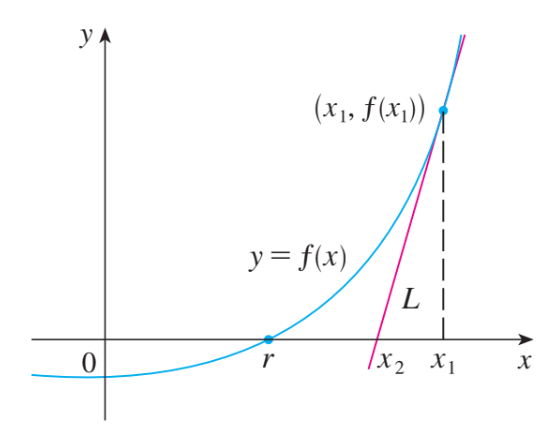
\includegraphics[width=0.4\linewidth]{pic/sec2_1.png}\vspace{0.5cm}\caption{Đồ thị hàm số phi tuyến bất kỳ \cite{stewart2008}} \label{fig:1}\end{figure}\end{center}

\begin{center}\begin{figure}[h]\centering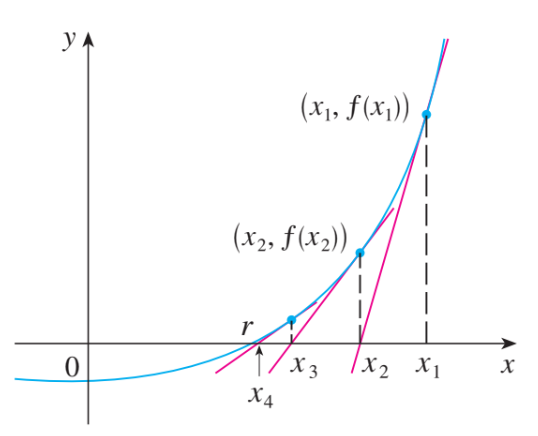
\includegraphics[width=0.4\linewidth]{pic/sec2_2.png}\vspace{0.5cm}\caption{Quá trình hội tụ của nghiệm xấp xỉ qua các bước lặp \cite{stewart2008}}
\label{fig:sec2_2}
\label{fig:2}\end{figure}\end{center}
% 

Để làm cơ sở định lượng chặt chẽ cho trực giác hình học này, ta sử dụng khai triển chuỗi Taylor của hàm $f(x)$ tại lân cận điểm $x_n$:
\begin{equation}
    f(x) \approx f(x_n) + f'(x_n)(x - x_n) + \frac{f''(\xi)}{2!}(x - x_n)^2
    \label{eq:taylor_1d}
\end{equation}
với $\xi$ là một điểm nằm giữa $x$ và $x_n$. Bằng cách tuyến tính hóa hàm số — tức là bỏ qua số hạng bậc hai và các số hạng bậc cao hơn khi $x$ đủ gần $x_n$ — ta thu được biểu thức xấp xỉ tuyến tính (chính là phương trình đường tiếp tuyến $L(x)$):
\begin{equation}
    f(x) \approx L(x) = f(x_n) + f'(x_n)(x - x_n)
\end{equation}
Nghiệm của phương trình phi tuyến $f(x)=0$ lúc này được xấp xỉ bằng nghiệm của phương trình tuyến tính $L(x)=0$. Để tìm điểm xấp xỉ tiếp theo $x_{n+1}$, ta cho $L(x_{n+1}) = 0$:
\begin{equation}
    0 = f(x_n) + f'(x_n)(x_{n+1} - x_n)
\end{equation}
Vì $f'(x_n) \neq 0$, ta chuyển vế và rút ra được \textbf{công thức lặp Newton–Raphson}:
\begin{equation}
    \boxed{x_{n+1} = x_n - \frac{f(x_n)}{f'(x_n)}}, \qquad n = 0, 1, 2, \ldots
    \label{eq:newton_1d}
\end{equation}

Để đảm bảo dãy số $\{x_n\}$ hội tụ về nghiệm $\alpha$, điểm xuất phát $x_0 \in [a,b]$ cần được chọn theo \textbf{điều kiện Fourier}: $f(x_0) \cdot f''(x_0) > 0$ \cite{dau2026hephuongtrinh}.

% Về mặt hình học, phương pháp Newton–Raphson tiếp cận nghiệm bằng cách thay thế đồ thị hàm số $y = f(x)$ bằng tiếp tuyến của nó tại điểm xấp xỉ hiện tại. Để làm cơ sở định lượng chặt chẽ cho trực giác này, ta sử dụng khai triển chuỗi Taylor của hàm $f(x)$ tại lân cận điểm $x_n$:
% \begin{equation}
% f(x) = f(x_n) + f'(x_n)(x - x_n) + \frac{f''(\xi)}{2!}(x - x_n)^2
% \label{eq:taylor_1d}
% \end{equation}
% với $\xi$ là một điểm nằm giữa $x$ và $x_n$. Bằng cách tuyến tính hóa hàm số — tức là bỏ qua số hạng bậc hai và các số hạng bậc cao hơn khi $x$ đủ gần $x_n$ — ta thu được biểu thức xấp xỉ tuyến tính (đường tiếp tuyến):
% \begin{equation}
% f(x) \approx f(x_n) + f'(x_n)(x - x_n)
% \end{equation}
% Để tìm điểm xấp xỉ tiếp theo $x_{n+1}$, ta cho biểu thức xấp xỉ này bằng $0$:
% \begin{equation}
% f(x_n) + f'(x_n)(x_{n+1} - x_n) = 0
% \end{equation}
% Vì $f'(x_n) \neq 0$, ta rút ra được \textbf{công thức lặp Newton–Raphson}:
% \begin{equation}
% \boxed{x_{n+1} = x_n - \frac{f(x_n)}{f'(x_n)}}, \qquad n = 0, 1, 2, \ldots
% \label{eq:newton_formula_1d}
% \end{equation}
% Để đảm bảo dãy số $\{x_n\}$ hội tụ về nghiệm $\alpha$, điểm xuất phát $x_0 \in [a,b]$ cần được chọn theo \textbf{điều kiện Fourier}: $f(x_0) \cdot f''(x_0) > 0$ \cite{dau2026hephuongtrinh}.

% ─────────────────────────────────────────────────────────────
\subsubsection{Phân tích tính hội tụ}



% 


% Trong các phương pháp số, việc một thuật toán tạo ra dãy lặp chưa đủ để đảm bảo tìm được nghiệm đúng. Một thuật toán hiệu quả cần có khả năng hội tụ về nghiệm mong muốn với tốc độ đủ nhanh và ổn định. Cũng như là có thể đánh giá được độ phức tạp của chúng cho việc xem xét tài nguyên sử dụng và thời gian tính toán.

Trước hết ta cần chứng minh dãy $\{x_n\}$ hội tụ nếu ta chọn nghiệm theo điều kiện Fourier. Ta xét 1 đoạn đồ thị trên khoảng phân ly nghiệm $(a,b)$ thì nó sẽ có 4 trường hợp như hình dưới đây 

\begin{figure}[H]
    \centering
    \begin{subfigure}[b]{0.3\textwidth}
        \centering
        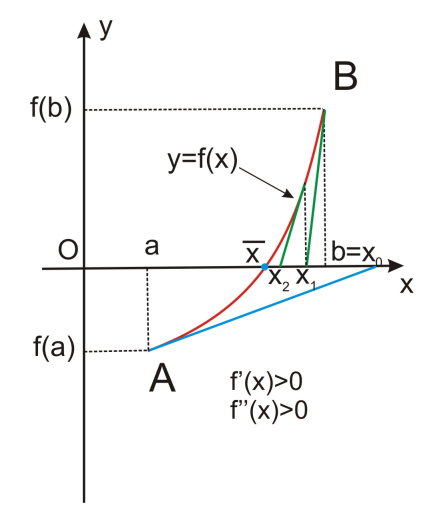
\includegraphics[width=\textwidth]{pic/ppt_sec1_1.png}
        \label{fig:a1}
        \caption{}
    \end{subfigure}
    \hfill
    \begin{subfigure}[b]{0.3\textwidth}
        \centering
        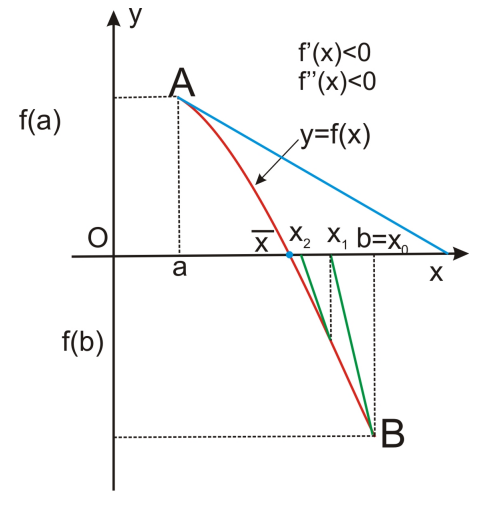
\includegraphics[width=\textwidth]{pic/ppt_sec1_2.png}
        \label{fig:b1}
        \caption{}
    \end{subfigure}
    \hfill
    \begin{subfigure}[b]{0.3\textwidth}
        \centering
        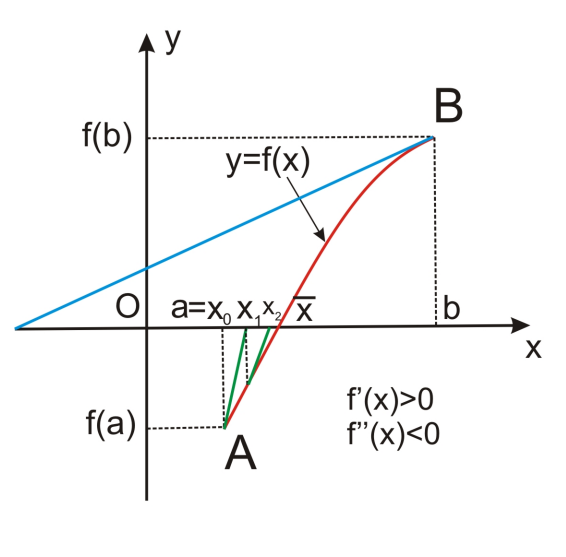
\includegraphics[width=\textwidth]{pic/ppt_sec1_3.png}
        \label{fig:c1}
        \caption{}
    \end{subfigure}
    \hfill
    \begin{subfigure}[b]{0.3\textwidth}
        \centering
        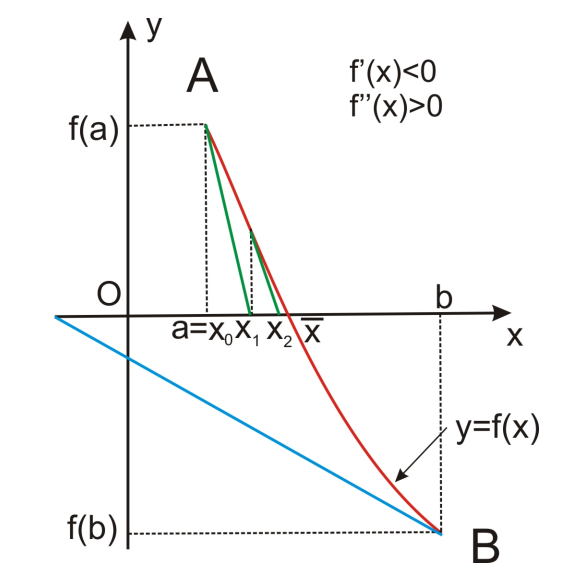
\includegraphics[width=\textwidth]{pic/ppt_sec1_4.png}
        \label{fig:d1}
        \caption{}
    \end{subfigure}
    
    \caption{Các trường hợp xảy ra Nguồn: \cite{dau2026hephuongtrinh}}
    \label{fig:ba-hinh}
\end{figure}

Xét hình (a) và (b) ta được 
$$a < \bar{x} < \dots < x_n < x_{n-1} < \dots < x_1 < x_0 = b$$

Và hình (c) và (d) sẽ cho ta được kết quả 

$$a = x_0 < x_1 < \dots < x_{n-1} < x_n < \dots < \bar{x} < b$$

Do đó với các trường hợp có thể của đồ thị thì thấy dãy đơn điệu và bị chặn. Do đó ta có được dãy hội tụ theo định lý Weierstrass.

% Độ hội tụ của một thuật toán lặp mô tả khả năng mà dãy nghiệm gần đúng sinh ra bởi thuật toán tiến dần đến nghiệm chính xác của bài toán. 

% Giả sử $\alpha$ là nghiệm đúng của hệ phương trình và $x_n$ là nghiệm gần đúng tại bước lặp thứ $n$, ta định nghĩa sai số tại bước lặp thứ $n$ là
% \[
% e_n = \|x_n-\alpha\|.
% \]

% Một thuật toán được gọi là hội tụ nếu
% \[
% \lim_{n\to\infty} e_n = 0.
% \]

% Ngoài việc xét thuật toán có hội tụ hay không, tốc độ giảm của sai số cũng là một yếu tố quan trọng. Trong phân tích số, tốc độ hội tụ thường được mô tả thông qua cấp hội tụ (order of convergence), được xác định bởi quan hệ
% \[
% e_{n+1}\approx Ce_n^p,
% \]
% với $C>0$ và $p$ được gọi là cấp hội tụ của thuật toán.

% Nếu $p=1$ thì hệ hội tụ tuyến tính, còn nếu $p=2$ thì thuật toán có hội tụ bậc hai. Phương pháp Newton là một ví dụ tiêu biểu của thuật toán có hội tụ bậc hai khi giá trị khởi tạo đủ gần nghiệm đúng.

% \textbf{Chứng minh ~\cite{chapra_ch6}:}
% Ta gọi $\alpha$ là nghiệm chính xác, tức $f(\alpha) = 0$. Tại bước lặp thứ $n$. Khi đó ta có sai số tại $n$ 

% \begin{equation}
%     e_n = x_n - \alpha \quad \implies \quad \alpha = x_n - e_n.
%     \label{eq:error_def}
% \end{equation}


% Khai triển Taylor của $f$ tại $x_n$, đánh giá tại $\alpha$ và dùng $f(\alpha) = 0$:

% \begin{equation}
%     0 = f(x_n) + f'(x_n)\,(\alpha - x_n) + \frac{f''(\xi)}{2}\,(\alpha - x_n)^2,
%     \label{eq:conv_taylor}
% \end{equation}

% trong đó $\xi$ nằm giữa $x_n$ và $\alpha$. Thay $\alpha - x_n = -e_n$:

% \begin{equation}
%     0 = f(x_n) - e_n f'(x_n) + \frac{e_n^2}{2}\, f''(\xi).
%     \label{eq:conv_taylor2}
% \end{equation}

% Chia cho $f'(x_n) \neq 0$:

% \begin{equation}
%     0 = \frac{f(x_n)}{f'(x_n)} - e_n + \frac{f''(\xi)}{2f'(x_n)}\, e_n^2.
%     \label{eq:conv_div}
% \end{equation}

% Từ công thức lặp \eqref{eq:newton_1d}, trừ cả hai vế cho $\alpha$:

% \begin{equation}
%     e_{n+1} = x_{n+1} - \alpha = e_n - \frac{f(x_n)}{f'(x_n)}.
%     \label{eq:error_recur}
% \end{equation}

% Kết hợp \eqref{eq:conv_div} và \eqref{eq:error_recur}:

% \begin{equation}
%     \boxed{e_{n+1} = \frac{f''(\xi)}{2\,f'(x_n)}\, e_n^2.}
%     \label{eq:quadratic_convergence}
% \end{equation}

% Hệ thức chứng minh \textbf{tính hội tụ bậc hai} của phương pháp Newton–Raphson: sai số ở bước tiếp theo tỷ lệ với \textit{bình phương} sai số hiện tại. Nếu $|e_n| \approx 10^{-2}$, thì $|e_{n+1}| \approx 10^{-4}$, rồi $10^{-8}$, v.v.

Để đánh giá tốc độ giảm của sai số, trong phân tích số người ta thường sử dụng khái niệm \textit{cấp hội tụ} (order of convergence). Gọi sai số tại bước lặp thứ $n$ là $e_n = x_n - \alpha$. Nếu tồn tại hằng số $C > 0$ và số thực $p \ge 1$ sao cho:
\begin{equation}
    |e_{n+1}| \approx C |e_n|^p
\end{equation}
thì $p$ được gọi là cấp hội tụ. Với phương pháp Newton–Raphson 1 ẩn, ta sẽ chứng minh thuật toán đạt cấp hội tụ $p = 2$ (hội tụ bậc hai) khi điểm khởi tạo đủ gần nghiệm \cite{chapra_ch6}.

\textbf{Chứng minh:}
Ta có nghiệm chính xác là $\alpha$, tức $f(\alpha) = 0$. Sai số tại bước lặp thứ $n$ được xác định bởi:
\begin{equation}
    e_n = x_n - \alpha \quad \implies \quad \alpha = x_n - e_n.
    \label{eq:error_def}
\end{equation}
Khai triển chuỗi Taylor của hàm số $f$ tại lân cận $x_n$, đánh giá tại điểm $\alpha$ và kết hợp điều kiện $f(\alpha) = 0$, ta có:
\begin{equation}
    0 = f(\alpha) = f(x_n) + f'(x_n)\,(\alpha - x_n) + \frac{f''(\xi)}{2}\,(\alpha - x_n)^2,
    \label{eq:conv_taylor}
\end{equation}
trong đó $\xi$ là một điểm nằm giữa $x_n$ và $\alpha$. Thay $\alpha - x_n = -e_n$ vào \eqref{eq:conv_taylor}:
\begin{equation}
    0 = f(x_n) - e_n f'(x_n) + \frac{e_n^2}{2}\, f''(\xi).
    \label{eq:conv_taylor2}
\end{equation}
Chia cả hai vế cho $f'(x_n) \neq 0$:
\begin{equation}
    0 = \frac{f(x_n)}{f'(x_n)} - e_n + \frac{f''(\xi)}{2f'(x_n)}\, e_n^2.
    \label{eq:conv_div}
\end{equation}
Mặt khác, từ công thức lặp Newton–Raphson \eqref{eq:newton_1d}, trừ cả hai vế cho $\alpha$ để thiết lập hệ thức truy hồi cho sai số:
\begin{equation}
    x_{n+1} - \alpha = x_n - \alpha - \frac{f(x_n)}{f'(x_n)} \quad \implies \quad e_{n+1} = e_n - \frac{f(x_n)}{f'(x_n)}.
    \label{eq:error_recur}
\end{equation}
Từ \eqref{eq:error_recur}, ta suy ra $e_n - e_{n+1} = \frac{f(x_n)}{f'(x_n)}$. Thay thế đại lượng này vào phương trình \eqref{eq:conv_div}, ta thu được:
\begin{equation}
    \boxed{e_{n+1} = \frac{f''(\xi)}{2\,f'(x_n)}\, e_n^2.}
    \label{eq:quadratic_convergence}
\end{equation}

\textbf{Kết luận:} Hệ thức \eqref{eq:quadratic_convergence} chứng minh rõ ràng tính hội tụ bậc hai của phương pháp Newton–Raphson, vì sai số ở bước lặp tiếp theo tỷ lệ thuận với bình phương sai số của bước trước đó. Nếu tại một bước lặp sai số đạt $|e_n| \approx 10^{-2}$, thì ở các bước tiếp theo sai số sẽ giảm cực nhanh theo cấp số mũ: $|e_{n+1}| \approx 10^{-4}$, rồi $10^{-8}$, $10^{-16}$, v.v.

\begin{bt}{Ví dụ}
    Cho phương trình $f(x) = x^3 - 3x + 1$ trong khoảng cách ly nghiệm $[0;\, 0{,}5]$. Tìm nghiệm gần đúng $x_3$ bằng phương pháp Newton–Raphson.
\end{bt}
\noindent{\textbf{Giải.}}

Ta có $f(0) > 0$, $f(0{,}5) < 0$, $f'(x) = 3x^2 - 3 < 0$ với mọi $x\in[0;\,0{,}5]$, và $f''(x) = 6x \geq 0$ với mọi $x\in[0;\,0{,}5]$, nên theo điều kiện Fourier ta chọn $x_0 = 0$.

Áp dụng công thức lặp \eqref{eq:newton_1d}:

\begin{equation}
    x_n = x_{n-1} - \frac{f(x_{n-1})}{f'(x_{n-1})}
        = x_{n-1} - \frac{x_{n-1}^3 - 3x_{n-1} + 1}{3x_{n-1}^2 - 3}
        = \frac{2x_{n-1}^3 - 1}{3x_{n-1}^2 - 3}.
    \label{eq:example_iter}
\end{equation}

\begin{table}[h]
\centering
\begin{tabular}{|c|c|c|}
\hline
$n$ & $x_n$ & $\Delta x_n = |x_n - x_{n-1}|$ \\
\hline
1 & 0.3333333333 & 3.33333333e-01 \\
\hline
2 & 0.3472222222 &1.38888889e-02 \\
\hline
3 & 0.3472963532 &7.41309416e-05\\
\hline
4 & 0.3472963553 &2.16999265e-09\\
\hline
\end{tabular}
\end{table}


\subsection{ Mở rộng cho hệ phương trình phi tuyến $n$ biến}

Một câu hỏi quan trọng được đặt ra: Làm thế nào để giải quyết các bài toán thực tế khi không chỉ có một biến số mà là một hệ gồm $n$ phương trình với $n$ ẩn số?

Về mặt trực giác, nếu ở không gian $Oxy$ ta dùng \textbf{đường tiếp tuyến} để xấp xỉ đường cong, thì ở không gian nhiều 3 chiều ta sẽ dùng các \textbf{mặt phẳng tiếp diện} để xấp xỉ các mặt cong phức tạp tại điểm dự đoán ban đầu.

% ─────────────────────────────────────────────────────────────

\subsubsection{Nội dung phương pháp cho $n$ chiều}

Xét hệ $n$ phương trình $n$ biến:

\begin{equation}
    \begin{cases}
        f_1(x_1, x_2, \dots, x_n) = 0, \\
        f_2(x_1, x_2, \dots, x_n) = 0, \\
        \quad \vdots \\
        f_n(x_1, x_2, \dots, x_n) = 0.
    \end{cases}
    \label{eq:system}
\end{equation}

Giả sử các hàm $f_i$ ($i = \overline{1,n}$) và các đạo hàm riêng của chúng đến bậc hai đều liên tục và tồn tại. Khai triển Taylor bậc nhất của $f_i$ tại lân cận điểm $(x_1,\dots,x_n)$:

\begin{equation}
   f_i(x_1 +h_1,\dots,x_n+h_n) \approx f_i(x_1,\dots,x_n) + h_1\dfrac{\partial f_i (x_1,\dots,x_n)}{\partial x_1} + \dots + h_n\dfrac{\partial f_i (x_1,\dots,x_n)}{\partial x_n}
   \label{eq:taylor_system}
\end{equation}

Gộp $n$ khai triển \eqref{eq:taylor_system} lại, ta được hệ phương trình:
\begin{equation}
\begin{cases}
 f_1(x_1 +h_1,\dots,x_n+h_n) \approx f_1(x_1,\dots,x_n) + h_1\dfrac{\partial f_1 (x_1,\dots,x_n)}{\partial x_1} + \dots + h_n\dfrac{\partial f_1 (x_1,\dots,x_n)}{\partial x_n} \\
 f_2(x_1 +h_1,\dots,x_n+h_n) \approx f_2(x_1,\dots,x_n) + h_1\dfrac{\partial f_2 (x_1,\dots,x_n)}{\partial x_1} + \dots + h_n\dfrac{\partial f_2 (x_1,\dots,x_n)}{\partial x_n} \\
 \quad \vdots \\
 f_n(x_1 +h_1,\dots,x_n+h_n) \approx f_n(x_1,\dots,x_n) + h_1\dfrac{\partial f_n (x_1,\dots,x_n)}{\partial x_1} + \dots + h_n\dfrac{\partial f_n (x_1,\dots,x_n)}{\partial x_n}
\end{cases}
\label{eq:linear_system}
\end{equation}

Ta đặt vector trạng thái hiện tại là $\mathbf{x}^{(0)} = (x_1,\dots,x_n)^\top$, vector trạng thái mới là $\mathbf{x}^{(1)} = (x_1+h_1,\dots,x_n+h_n)^\top$, và vector bước lặp là $\mathbf{h} = (h_1, h_2, \dots, h_n)^\top$. 

Hệ \eqref{eq:linear_system} có thể được viết gọn lại dưới dạng ma trận:

\begin{equation}
    \mathbf{F}(\mathbf{x}^{(1)}) \approx \mathbf{F}(\mathbf{x}^{(0)}) + \mathbf{J}(\mathbf{x}^{(0)}) \mathbf{h}
    \label{eq:matrix_form}
\end{equation}

Trong đó, $\mathbf{F}(\mathbf{x})$ là vector chứa các hàm $f_i$, và $\mathbf{J}(\mathbf{x}^{(0)})$ là \textbf{ma trận Jacobian} cấp $n \times n$ được định nghĩa như sau:
\begin{equation}
    \mathbf{J}(\mathbf{x}^{(0)}) =
    \begin{pmatrix}
        \dfrac{\partial f_1}{\partial x_1} & \dfrac{\partial f_1}{\partial x_2} & \cdots & \dfrac{\partial f_1}{\partial x_n} \\[8pt]
        \dfrac{\partial f_2}{\partial x_1} & \dfrac{\partial f_2}{\partial x_2} & \cdots & \dfrac{\partial f_2}{\partial x_n} \\[4pt]
        \vdots & \vdots & \ddots & \vdots \\[4pt]
        \dfrac{\partial f_n}{\partial x_1} & \dfrac{\partial f_n}{\partial x_2} & \cdots & \dfrac{\partial f_n}{\partial x_n}
    \end{pmatrix}_{\!\mathbf{x} = \mathbf{x}^{(0)}}
    \label{eq:jacobian_def}
\end{equation}

Xét cho $\mathbf{F}(\mathbf{x}^{(1)}) = \mathbf{0}$ khi đó ta được $\mathbf{h = x^{(1)} - x^{(0)}} $

Thay vào phương trình \eqref{eq:matrix_form}, ta có:
\begin{equation}
    \mathbf{0} \approx \mathbf{F}(\mathbf{x}^{(0)}) + \mathbf{J}(\mathbf{x}^{(0)}) \mathbf{h}
\end{equation}

Chuyển vế, ta thu được hệ phương trình đại số tuyến tính đối với vector ẩn $\mathbf{h}$:
\begin{equation}
    \mathbf{J}(\mathbf{x}^{(0)}) \mathbf{h} = -\mathbf{F}(\mathbf{x}^{(0)})
    \label{eq:solve_h}
\end{equation}

Giả sử ma trận Jacobian $\mathbf{J}(\mathbf{x}^{(0)})$ không suy biến (tức là $\det(\mathbf{J}) \neq 0$), ta có thể tìm được $\mathbf{h}$ bằng cách nhân cả hai vế với ma trận nghịch đảo $\mathbf{J}^{-1}(\mathbf{x}^{(0)})$:
\begin{equation}
    \mathbf{h} = -[\mathbf{J}(\mathbf{x}^{(0)})]^{-1} \mathbf{F}(\mathbf{x}^{(0)})
\end{equation}

Vì $\mathbf{x}^{(1)} = \mathbf{x}^{(0)} + \mathbf{h}$, ta suy ra trạng thái ở bước tiếp theo:
\begin{equation}
    \mathbf{x}^{(1)} = \mathbf{x}^{(0)} - [\mathbf{J}(\mathbf{x}^{(0)})]^{-1} \mathbf{F}(\mathbf{x}^{(0)})
\end{equation}

Khái quát hóa quá trình này cho bước lặp thứ $k$ (với $k = 0, 1, 2, \dots$), ta nhận được \textbf{công thức lặp Newton-Raphson} dạng tổng quát:
\begin{equation}
    \mathbf{x}^{(k+1)} = \mathbf{x}^{(k)} - [\mathbf{J}(\mathbf{x}^{(k)})]^{-1} \mathbf{F}(\mathbf{x}^{(k)})
    \label{eq:newton_raphson_general}
\end{equation}

% Xét hệ $n$ phương trình $n$ biến:

% \begin{equation}
%     \begin{cases}
%         f_1(x_1, x_2, \dots, x_n) = 0, \\
%         f_2(x_1, x_2, \dots, x_n) = 0, \\
%         \quad \vdots \\
%         f_n(x_1, x_2, \dots, x_n) = 0.
%     \end{cases}
%     \label{eq:system}
% \end{equation}

% Giả sử các hàm $f_i$ ($i = \overline{1,n}$) và các đạo hàm riêng của chúng đến bậc hai đều liên tục và tồn tại. Khai triển Taylor của $f_i$ tại lân cận điểm $(x_1,\dots,x_n)$ 

% \begin{equation}
%    f_i(x_1 +h_1,\dots,x_n+h_n) = f_i(x_1,\dots,x_n)+h_1.\dfrac{\partial f_i (x_1,\dots,x_n)}{x_1} +...+h_n. \dfrac{\partial f_i (x_1,\dots,x_n)}{x_n}
%    \label{eq:taylor_system}
% \end{equation}

% Gộp $n$ hệ \eqref{eq:taylor_system}  lại ta viết thành dạng ma trận:
% \begin{equation}
% \begin{cases}
%  f_1(x_1 +h_1,\dots,x_n+h_n) = f_1(x_1,\dots,x_n)+h_1.\dfrac{\partial f_1 (x_1,\dots,x_n)}{\partial x_1} +...+h_n. \dfrac{\partial f_1 (x_1,\dots,x_n)}{\partial x_n}\\
%   f_2(x_1 +h_1,\dots,x_n+h_n) = f_2(x_1,\dots,x_n)+h_1.\dfrac{\partial f_2 (x_1,\dots,x_n)}{\partial x_1} +...+h_n. \dfrac{\partial f_2 (x_1,\dots,x_n)}{\partial x_n} \\
%   \dots \\
%    f_n(x_1 +h_1,\dots,x_n+h_n) = f_n(x_1,\dots,x_n)+h_1.\dfrac{\partial f_n (x_1,\dots,x_n)}{\partial x_1} +...+h_n. \dfrac{\partial f_n (x_1,\dots,x_n)}{\partial x_n}
    
%     \label{eq:linear_system}
% \end{cases}
% \end{equation}

% Ta đặt $\mathbf{x^{(0)}}= (x_1,\dots,x_n)$ và $\mathbf{x^{(1)}}= (x_1+h_1,\dots,x_n+h_n)$.

% Hay viết gọn dưới dạng vector: $\mathbf{F}(\mathbf{x^{(0)}}) = \begin{bmatrix}
%     f_1(x_1,\dots,x_n)\\
%     f_2(x_1,\dots,x_n)\\
%     \vdots \\
%     f_n(x_1,\dots,x_n)
% \end{bmatrix} $. Ta rút gọn hệ \ref{eq:linear_system} lại thành các ma trận nhân nhau và với ẩn $\mathbf{h} = (h_1, h_2, \dots, h_n)^\top$ ta được

% \begin{equation}
%     \mathbf{F(x^{(1)})} = \mathbf{F(x^{(0)})} +\mathbf{J}(\mathbf{x}^{(0)}).\mathbf{h}
% \end{equation}


% trong đó $\mathbf{J}(\mathbf{x}^{(0)})$ là \textbf{ma trận Jacobian} cấp $n\times n$:
% \begin{equation}
%     \mathbf{J}(\mathbf{x}^{(0)}) =
%     \begin{pmatrix}
%         \dfrac{\partial f_1}{\partial x_1} & \dfrac{\partial f_1}{\partial x_2} & \cdots & \dfrac{\partial f_1}{\partial x_n} \\[8pt]
%         \dfrac{\partial f_2}{\partial x_1} & \dfrac{\partial f_2}{\partial x_2} & \cdots & \dfrac{\partial f_2}{\partial x_n} \\[4pt]
%         \vdots & \vdots & \ddots & \vdots \\[4pt]
%         \dfrac{\partial f_n}{\partial x_1} & \dfrac{\partial f_n}{\partial x_2} & \cdots & \dfrac{\partial f_n}{\partial x_n}
%     \end{pmatrix}_{\!\mathbf{x} = \mathbf{x}^{(0)}}.
%     \label{eq:jacobian_def}
% \end{equation}

Nếu $\mathbf{J}(\mathbf{x}^{(0)})$ khả nghịch, nghiệm của \eqref{eq:linear_system} là:

\begin{equation}
    \mathbf{h} = -\mathbf{J}^{-1}\!\left(\mathbf{x}^{(0)}\right)\, \mathbf{F}\!\left(\mathbf{x}^{(0)}\right).
    \label{eq:h_solution}
\end{equation}

Do đó, điểm xấp xỉ tiếp theo là:

\begin{equation}
    \mathbf{x}^{(k+1)} = \mathbf{x}^{(k)} - \mathbf{J}^{-1}\!\left(\mathbf{x}^{(k)}\right)\, \mathbf{F}\!\left(\mathbf{x}^{(k)}\right), \qquad k = 0,1,2,\ldots
    \label{eq:newton_nd}
\end{equation}

Quá trình lặp lại: tính $\mathbf{J}(\mathbf{x}^{(k+1)})$ và tiếp tục cho đến khi $\mathbf{x}$ hội tụ.

Thay vì tìm giao điểm của các mặt cong phi tuyến phức tạp, thuật toán liên tục xấp xỉ chúng bằng các mặt phẳng tiếp tuyến — một bài toán tuyến tính đơn giản hơn nhiều.

Khi này ta có phát biểu tổng quát hơn và chặt chẽ hơn.


\begin{bt}{Phương pháp Newton cho hệ phương trình phi tuyến}
Xét hệ phương trình phi tuyến:
$$
\mathbf{F}(\mathbf{x})=\mathbf{0}
$$
với $\mathbf{F}: D \subset \mathbb{R}^n \rightarrow \mathbb{R}^n$, trong đó $D$ là một tập mở.

Giả sử $\mathbf{F}$ là hàm khả vi liên tục trên $D$ và ma trận Jacobian $\mathbf{J}\!\left(\mathbf{x}^{(k)}\right)$ không suy biến (khả nghịch) tại mọi bước lặp $k$. 
Bắt đầu từ vector khởi tạo $\mathbf{x}^{(0)} \in D$, giả sử mọi xấp xỉ $\mathbf{x}^{(k)}$ đều thuộc $D$, dãy lặp Newton được xác định bởi công thức:
\begin{equation}
    \mathbf{x}^{(k+1)}
    =
    \mathbf{x}^{(k)}
    -
    \mathbf{J}^{-1}\!\left(\mathbf{x}^{(k)}\right)\mathbf{F}\!\left(\mathbf{x}^{(k)}\right), \quad k = 0, 1, 2, \dots
\end{equation}
\end{bt}

% \begin{bt}{Ví dụ}
%      Cho hệ phương trình:
% $$
% \begin{cases} 
% u(x, y) = x^2 + xy - 10 = 0 \\ 
% v(x, y) = y + 3xy^2 - 57 = 0 
% \end{cases} 
% $$
% cho biết nghiệm chính xác $(x = 2, y = 3)$.\\
% Nghiệm ban đầu cho $(x_0 = 1{,}5; y_0 = 3{,}5)$.

% \end{bt}
% \textbf{Giải}

% Ta tính các đạo hàm riêng (các phần tử của ma trận Jacobian):
% $$
% \begin{aligned}
% \frac{\partial v}{\partial y} &= 1 + 6xy &\implies \frac{\partial v_0}{\partial y_0} &= 1 + 6(1{,}5)(3{,}5) = 32{,}5 \\
% \frac{\partial v}{\partial x} &= 3y^2 &\implies \frac{\partial v_0}{\partial x_0} &= 3(3{,}5)^2 = 36{,}75 \\
% \frac{\partial u}{\partial y} &= x &\implies \frac{\partial u_0}{\partial y_0} &= 1{,}5 \\
% \frac{\partial u}{\partial x} &= 2x + y &\implies \frac{\partial u_0}{\partial x_0} &= 2(1{,}5) + 3{,}5 = 6{,}5
% \end{aligned}
% $$

% Định thức Jacobian: 
% $$ 
% \det J_0 = \frac{\partial u_0}{\partial x_0}\frac{\partial v_0}{\partial y_0} - \frac{\partial u_0}{\partial y_0}\frac{\partial v_0}{\partial x_0} = 6{,}5(32{,}5) - 1{,}5(36{,}75) = 156{,}125 
% $$

% Giá trị các hàm tại điểm ban đầu $(x_0, y_0)$:
% $$
% \begin{aligned}
% u_0 &= (1{,}5)^2 + 1{,}5(3{,}5) - 10 = -2{,}5 \\
% v_0 &= 3{,}5 + 3(1{,}5)(3{,}5)^2 - 57 = 1{,}625
% \end{aligned}
% $$

% Áp dụng công thức Newton-Raphson cho hệ phương trình, ta có bước 1 ($n=1$):
% $$
% \begin{cases}
% x_1 = x_0 - \dfrac{u_0 \frac{\partial v_0}{\partial y_0} - v_0 \frac{\partial u_0}{\partial y_0}}{\det J_0} = 1{,}5 - \dfrac{-2{,}5(32{,}5) - 1{,}625(1{,}5)}{156{,}125} \approx 2{,}03603 \\[15pt]
% y_1 = y_0 - \dfrac{v_0 \frac{\partial u_0}{\partial x_0} - u_0 \frac{\partial v_0}{\partial x_0}}{\det J_0} = 3{,}5 - \dfrac{1{,}625(6{,}5) - (-2{,}5)(36{,}75)}{156{,}125} \approx 2{,}84388
% \end{cases}
% $$

% Tiếp tục các bước xấp xỉ tương tự, nghiệm sẽ dần hội tụ về $(x = 2, y = 3)$.

% \vspace{1cm}
% \textbf{Bảng tổng hợp kết quả các bước lặp:}
% \vspace{0.3cm}

% \begin{center}
% \renewcommand{\arraystretch}{1.5}
% \begin{tabular}{|c|c|c|c|c|c|c|}
% \hline
% $n$ & $x_n$ & $y_n$ & $u(x_n, y_n)$ & $v(x_n, y_n)$ & $\Delta x_n = |x_n - x_{n-1}|$ & $\Delta y_n = |y_n - y_{n-1}|$ \\
% \hline
% 0 & $1{,}50000$ & $3{,}50000$ & $-2{,}50000$ & $1{,}62500$ & --- & --- \\
% \hline
% 1 & $2{,}03603$ & $2{,}84388$ & $-0{,}06437$ & $-4{,}75621$ & $0{,}53603$ & $0{,}65612$ \\
% \hline
% 2 & $1{,}99870$ & $3{,}00229$ & $-0{,}00452$ & $0{,}04957$ & $0{,}03733$ & $0{,}15841$ \\
% \hline
% 3 & $2{,}00000$ & $3{,}00000$ & $0{,}00000$ & $0{,}00000$ & $0{,}00130$ & $0{,}00229$ \\
% \hline
% \end{tabular}
% \end{center}
% ─────────────────── ──────────────────────────────────────────
% \subsection{Ma trận Jacobian}

% \begin{itemize}
%     \item Ma trận Jacobian là công cụ cốt lõi trong giải tích nhiều biến và giải tích vector.
%     \item Khi chuyển từ hàm một biến sang hàm vector nhiều biến, khái niệm đạo hàm cần được mở rộng để phản ánh sự thay đổi đồng thời của nhiều thành phần.
%     \item Ma trận Jacobian chính là sự tổng quát hóa của đạo hàm . Ý nghĩa hình học của nó là dùng một ma trận để xấp xỉ tuyến tính hàm số tại một điểm 
% \end{itemize}

% \textbf{a) Định nghĩa.~\cite{wikipedia_jacobian}}

% Cho $\mathbf{f} : \mathbb{R}^n \to \mathbb{R}^m$ sao cho mỗi đạo hàm riêng bậc nhất tồn tại trên $\mathbb{R}^n$. Hàm nhận $\mathbf{x} = (x_1,\dots,x_n)^\top \in \mathbb{R}^n$ và trả về $\mathbf{f}(\mathbf{x}) = (f_1(\mathbf{x}),\dots,f_m(\mathbf{x}))^\top \in \mathbb{R}^m$. Ma trận Jacobian $\mathbf{J}_{\mathbf{f}}$ là ma trận cấp $m \times n$ chứa tất cả đạo hàm riêng của hàm số :

% \begin{equation}
%     \mathbf{J}_{\mathbf{f}} =
%     \begin{bmatrix}
%         \nabla^\top f_1 \\ \vdots \\ \nabla^\top f_m
%     \end{bmatrix}
%     =
%     \begin{bmatrix}
%         \dfrac{\partial f_1}{\partial x_1} & \cdots & \dfrac{\partial f_1}{\partial x_n} \\[8pt]
%         \vdots & \ddots & \vdots \\[4pt]
%         \dfrac{\partial f_m}{\partial x_1} & \cdots & \dfrac{\partial f_m}{\partial x_n}
%     \end{bmatrix},
%     \label{eq:jacobian_full}
% \end{equation}

% trong đó $\nabla^\top f_i$ là gradient hàng (chuyển vị của gradient) của thành phần $f_i$.

% \textbf{Ví dụ 1.~\cite{wikipedia_jacobian}} Xét $\mathbf{F} : \mathbb{R}^2 \to \mathbb{R}^3$ với
% \begin{equation}
%     \mathbf{F}(x, y) =
%     \begin{bmatrix} x^2 y \\ 5x + \sin y \\ 4y \end{bmatrix}.
%     \label{eq:example_f}
% \end{equation}
% Ma trận Jacobian của $\mathbf{F}$:
% \begin{equation}
%     \mathbf{J}_{\mathbf{F}}(x,y) =
%     \begin{bmatrix}
%         2xy  & x^2 \\
%         5    & \cos y \\
%         0    & 4
%     \end{bmatrix}.
%     \label{eq:example_J}
% \end{equation}

% \textbf{b) Ý nghĩa hình học và xấp xỉ tuyến tính. ~\cite{wikipedia_jacobian}}

% Giả sử $\mathbf{F} : \mathbb{R}^n \to \mathbb{R}^m$ khả vi tại $\mathbf{p}$. Phép xấp xỉ tuyến tính tốt nhất của $\mathbf{f}$ trong lân cận $\mathbf{p}$:

% \begin{equation}
%     \mathbf{F}(\mathbf{x}) = \mathbf{F}(\mathbf{p}) + \mathbf{J}_{\mathbf{F}}(\mathbf{p})\,(\mathbf{x} - \mathbf{p}) + o\!\left(\|\mathbf{x}-\mathbf{p}\|\right)
%     \label{eq:linear_approx_nd}
% \end{equation}

% Đối với hàm một biến $f:\mathbb{R}\to\mathbb{R}$, \eqref{eq:linear_approx_nd} thu gọn về đa thức Taylor bậc nhất (phương trình tiếp tuyến):
% \begin{equation}
%     f(x) = f(p) + f'(p)\,(x-p) + o(x-p).
%     \label{eq:taylor_1d_approx}
% \end{equation}

% \begin{itemize}
%     \item Trong không gian 1 chiều: $f'(p)$ là hệ số góc của đường tiếp tuyến tại điểm $p$ tạo ra \textbf{đường thẳng tiếp tuyến}.
%     \item Trong không gian $n$ chiều: $\mathbf{J}_{\mathbf{f}}(\mathbf{p})$ cũng tương tự nhưng sẽ là gradient của hàm số và tạo ra \textbf{không gian tiếp xúc} (mặt phẳng tiếp diện).
% \end{itemize}

% \textbf{Ví dụ 2.} Xét $\mathbf{F}(x,y) = \begin{bmatrix} x^2+y \\ 2xy \end{bmatrix}$.
% Ma trận Jacobian:
% \begin{equation}
%     \mathbf{J}(x,y) =
%     \begin{bmatrix} 2x & 1 \\ 2y & 2x \end{bmatrix};
%     \qquad
%     \mathbf{J}(1,1) =
%     \begin{bmatrix} 2 & 1 \\ 2 & 2 \end{bmatrix}.
%     \label{eq:jacobian_example2}
% \end{equation}

% Tại $(x_0,y_0) = (1,1)$: $\mathbf{F}(1,1) = \begin{bmatrix} 2 \\ 2 \end{bmatrix}$.

% Xấp xỉ tuyến tính tại $\Delta\mathbf{x} = (0{,}1,\,-0{,}1)^\top$:
% \begin{equation}
%     \mathbf{F}(1{,}1;\,0{,}9) \approx \mathbf{F}(1,1) + \mathbf{J}(1,1)\,\Delta\mathbf{x}
%     = \begin{bmatrix}2\\2\end{bmatrix} + \begin{bmatrix}2&1\\2&2\end{bmatrix}\begin{bmatrix}0{,}1\\-0{,}1\end{bmatrix}
%     = \begin{bmatrix}2{,}1\\2\end{bmatrix}.
%     \label{eq:linearization_example}
% \end{equation}

% Giá trị thực: $f_1(1{,}1;\,0{,}9) = 2{,}11$; $f_2(1{,}1;\,0{,}9) = 1{,}98$. Kết quả xấp xỉ rất sát, minh chứng sức mạnh của phép tuyến tính hóa.

% % ─────────────────────────────────────────────────────────────
% \subsubsection{ Phân tích tính hội tụ của thuật toán }

\subsubsection{Đánh giá sai số và điều kiện dừng}Trong phương pháp Newton không gian một chiều, sai số xấp xỉ giữa hai bước lặp liên tiếp được xác định đơn giản thông qua giá trị tuyệt đối của khoảng cách:\begin{equation}\Delta x = \left| x^{(k)} - x^{(k-1)} \right|\end{equation}Tuy nhiên, đối với hệ phương trình đa biến, nghiệm xấp xỉ tại mỗi bước lặp là các vector $\mathbf{x}^{(k)}$. Việc đánh giá sai số lúc này không thể chỉ dựa trên phép trừ vector đơn thuần, mà đòi hỏi việc sử dụng các \textbf{chuẩn (norms)} trong không gian vector để ánh xạ toàn bộ sai số của hệ thống thành một đại lượng vô hướng duy nhất.Gọi vector nghiệm tại bước lặp thứ $k$ là $\mathbf{x}^{(k)}$ và bước trước đó là $\mathbf{x}^{(k-1)}$. Vector sai số bước lặp được định nghĩa là:\begin{equation}\Delta\mathbf{x} = \mathbf{x}^{(k)} - \mathbf{x}^{(k-1)}\end{equation}Trong thực hành tính toán số, hai loại chuẩn sau đây thường được áp dụng phổ biến nhất để thiết lập tiêu chuẩn hội tụ (điều kiện dừng) cho thuật toán:\begin{itemize}\item \textbf{Chuẩn 1 (Norm 1) — Tổng sai số tuyệt đối:}Chuẩn 1 đánh giá tổng mức độ sai lệch của toàn bộ hệ thống bằng cách lấy tổng giá trị tuyệt đối các thành phần của vector sai số:\begin{equation}|| \Delta\mathbf{x} ||_ 1 = \sum_{i=1}^{n} \left| x_i^{(k)} - x_i^{(k-1)} \right|\end{equation}Tiêu chuẩn này thường được sử dụng khi các biến trong hệ phương trình có vai trò ngang hàng và ta quan tâm đến sự hội tụ tích lũy của toàn hệ thống.\item \textbf{Chuẩn vô cùng (Infinity Norm) — Sai số cực đại:}
Chuẩn vô cùng đánh giá sai số dựa trên thành phần có sự sai lệch lớn nhất trong vector:
\begin{equation}
    \| \Delta\mathbf{x} \|_\infty = \max_{1 \le i \le n} \left| x_i^{(k)} - x_i^{(k-1)} \right|
\end{equation}
Đây là điều kiện dừng an toàn và khắt khe nhất. Nếu ta thiết lập ngưỡng dung sai $\| \Delta\mathbf{x} \|_\infty < \varepsilon$ (ví dụ $\varepsilon = 10^{-4}$), điều này đảm bảo chắc chắn rằng \textit{không có bất kỳ một biến đơn lẻ nào} trong hệ có sai số vượt qua ngưỡng cho phép. Trong mô phỏng kỹ thuật, chuẩn vô cùng thường được ưu tiên để tránh hiện tượng hội tụ giả.
\end{itemize}

% \subsubsection{Độ phức tạp thuật toán}
% Trong tính toán số, \textbf{độ phức tạp thuật toán} là đại lượng đánh giá số phép toán CPU và dung lượng RAM mà thuật toán tiêu tốn khi kích thước bài toán (số lượng biến hay phương trình) tăng lên. Để ước tính đại lượng này, ta sử dụng \textbf{ký hiệu $\mathcal{O}$}. Cách đánh giá rất đơn giản: lập biểu thức tổng số phép toán cơ bản cấu thành nên thuật toán, sau đó chỉ giữ lại số hạng có bậc cao nhất và bỏ qua các hệ số tự do. Còn về độ phức tạp không gian sẽ đánh giá dung lượng bộ nhớ mà phép toán chiếm dụng.

% \textbf{Ví dụ:} Một khối lệnh có số phép toán (số lần tính cộng trừ nhân chia v.v) là $T(n) = \frac{2}{3}n^3 + 5n^2 + 10$, ta sẽ bỏ qua hằng số và số hạng bậc thấp hơn bậc cao nhất để kết luận độ phức tạp thời gian là $\mathcal{O}(n^3)$.

% Đánh giá phương pháp Newton Raphson gốc. 

% Tại mỗi bước lặp $k$, phương pháp Newton-Raphson quy bài toán về việc giải hệ phương trình tuyến tính:\begin{equation}\mathbf{J}\left(\mathbf{x}^{(k)}\right) \Delta\mathbf{x} = -\mathbf{F}\left(\mathbf{x}^{(k)}\right)\end{equation}Và để giải từ phi tuyến sang tuyến tính ta phải thực hiện hai bước sau. :\begin{enumerate}\item \textbf{Thiết lập ma trận Jacobian $\mathbf{J}$:} Ma trận có kích thước $n \times n$. Việc tính toán giá trị mới cho $n^2$ biểu thức đạo hàm riêng tại mỗi bước có độ phức tạp không gian là $\mathcal{O}(n^2)$.\item \textbf{Giải hệ phương trình tuyến tính:} Không ai đi tính trực tiếp ma trận nghịch đảo $\mathbf{J}^{-1}$ vì rủi ro sai số. Thay vào đó, máy tính dùng các thuật toán chuẩn như phép khử Gauss hoặc phân rã LU để tìm $\Delta\mathbf{x}$. Đối với một ma trận đầy đủ, các thuật toán này có \textbf{độ phức tạp thời gian là $\mathcal{O}(n^2)$}.\end{enumerate}.

 
\section{Các phương pháp giải hệ tuyến tính phổ biến.}
Ở đây ta sẽ chỉ nói qua về cách các thuật toán giải hệ hoạt động để có thể nhúng vào chương trình lập trình để có thể chạy được chứ không bàn về hay chứng minh lại cách mà phương pháp lặp hội tụ cũng như hội tụ như thế nào. 

% \subsection{Vấn đề của việc tính toán truyền thống}

% Trước tiên, ta xét hệ phương trình phi tuyến tổng quát sau đây:
% \begin{equation}
%     \begin{cases}
%         ... \\
%         ...
%     \end{cases}
% \end{equation}

% Có thể nhận thấy, việc giải hệ phương trình bằng các công thức lặp thông thường đòi hỏi khối lượng tính toán rất lớn. Đặc biệt, thao tác tính toán trực tiếp ma trận nghịch đảo Jacobian tại mỗi bước lặp tiêu tốn nhiều thời gian và hoàn toàn không tối ưu về mặt tài nguyên phần cứng.

% Hơn nữa, việc lựa chọn điểm xuất phát ban đầu hiện nay chủ yếu vẫn mang tính ngẫu nhiên, thiếu cơ sở toán học vững chắc, dẫn đến rủi ro thuật toán không thể hội tụ về đúng nghiệm mong muốn.

% Nhận thấy sau khi thực hiện xấp xỉ Newton Raphson, ta thu được 1 phương trình là 1 hệ tuyến tính nếu ta đã chọn điểm bắt đầu $\mathbf{x^{(0)}}$. Vì vậy mục tiêu tiếp theo ta sẽ tối ưu việc giải hệ tuyến tính này. Do đó, báo cáo cần tập trung cải thiện hai vấn đề cốt lõi:
% \begin{enumerate}
%     \item Bàn luận về việc chọn điểm ban đầu sao cho thuật toán lặp hiệu quả cũng như hội tụ về nghiệm cần thiết, thực tế.
%     \item Áp dụng phương pháp phân rã LU, lặp Jacobi để thay thế cho việc tìm nghịch đảo Jacobian, qua đó giải quyết bài toán đại số tuyến tính tại mỗi bước lặp một cách hiệu quả hơn.
% \end{enumerate}

% ==========================================
% KẾT THÚC MỤC 3.1 - BẮT ĐẦU MỤC 3.2
% ==========================================



% \subsection{Phương pháp LU}

% Cốt lõi của phương pháp phân rã LU là phân tích một ma trận hệ số $A$ thành tích của hai ma trận:
% $$ A = L \cdot U $$
% Trong đó, $L$ là ma trận tam giác dưới và $U$ là ma trận tam giác trên. Khi đó, việc giải hệ phương trình tuyến tính $A \cdot X = B$ được quy về việc giải tuần tự hai hệ phương trình tam giác đơn giản:
% $$ L \cdot Y = B \quad \text{và} \quad U \cdot X = Y $$

% Có nhiều phương pháp phân tích $A = L \cdot U$, tuy nhiên trong phạm vi báo cáo này, ta xét trường hợp ma trận $L$ có đường chéo chính bằng $1$, được gọi là thuật toán Doolittle. Khi đó, cấu trúc của hai ma trận có dạng:
% $$
% L = \begin{pmatrix} 1 & 0 & \dots & 0 \\ l_{21} & 1 & \dots & 0 \\ \vdots & \vdots & \ddots & \vdots \\ l_{n1} & l_{n2} & \dots & 1 \end{pmatrix}, \quad
% U = \begin{pmatrix} u_{11} & u_{12} & \dots & u_{1n} \\ 0 & u_{22} & \dots & u_{2n} \\ \vdots & \vdots & \ddots & \vdots \\ 0 & 0 & \dots & u_{nn} \end{pmatrix}
% $$

% Để xác định các phần tử của $L$ và $U$, ta dựa vào phương trình $A = L \cdot U$. Theo định nghĩa phép nhân ma trận, phần tử ở hàng $i$, cột $j$ của ma trận $A$ (ký hiệu là $a_{ij}$) bằng tích vô hướng của hàng $i$ trong ma trận $L$ và cột $j$ trong ma trận $U$:
% $$ a_{ij} = \sum_{k=1}^{n} l_{ik} u_{kj} $$

% Do đặc thù $L$ là ma trận tam giác dưới ($l_{ik} = 0$ khi $k > i$) và $U$ là ma trận tam giác trên ($u_{kj} = 0$ khi $k > j$), giới hạn của tổng sẽ thay đổi tùy thuộc vào vị trí của phần tử đang xét nằm ở nửa trên hay nửa dưới đường chéo chính.

% Trường hợp 1, xét việc tính các phần tử của ma trận $U$ ($i \le j$). Vì $i \le j$, các phần tử $l_{ik} = 0$ với mọi $k > i$. Do đó, tổng trên chỉ chạy đến $k = i$:
% $$ a_{ij} = \sum_{k=1}^{i} l_{ik} u_{kj} = \sum_{k=1}^{i-1} l_{ik} u_{kj} + l_{ii} u_{ij} $$
% Theo giả thiết của thuật toán Doolittle, các phần tử trên đường chéo của $L$ đều bằng 1 ($l_{ii} = 1$). Suy ra:
% $$ a_{ij} = \sum_{k=1}^{i-1} l_{ik} u_{kj} + u_{ij} \implies u_{ij} = a_{ij} - \sum_{k=1}^{i-1} l_{ik} u_{kj} \quad (1 < i \le j) $$
% Tại hàng đầu tiên ($i=1$), tổng phụ không tồn tại, ta có bước cơ sở $u_{1j} = a_{1j}$ với mọi $1 \le j \le n$.

% Trường hợp 2, xét việc tính các phần tử của ma trận $L$ ($i > j$). Vì $i > j$, các phần tử $u_{kj} = 0$ với mọi $k > j$. Do đó, tổng chỉ chạy đến $k = j$:
% $$ a_{ij} = \sum_{k=1}^{j} l_{ik} u_{kj} = \sum_{k=1}^{j-1} l_{ik} u_{kj} + l_{ij} u_{jj} $$
% Rút phần tử $l_{ij}$ ra từ phương trình trên, ta được:
% $$ l_{ij} = \frac{1}{u_{jj}} \left( a_{ij} - \sum_{k=1}^{j-1} l_{ik} u_{kj} \right) \quad (1 < j < i) $$
% Tại cột đầu tiên ($j=1$), tổng phụ không tồn tại, ta có bước cơ sở $l_{i1} = \frac{a_{i1}}{u_{11}}$ với mọi $2 \le i \le n$.

% Tổng hợp cả hai trường hợp, thuật toán nội suy tuần tự các phần tử của phân rã Doolittle được tóm tắt bằng hệ phương trình sau ~\cite{dau2026hephuongtrinh}:
% \begin{equation}
% \begin{cases}
%     u_{1j} = a_{1j} & (1 \le j \le n) \\
%     l_{i1} = \dfrac{a_{i1}}{u_{11}} & (2 \le i \le n) \\
%     u_{ij} = a_{ij} - \sum\limits_{k=1}^{i-1} l_{ik}u_{kj} & (1 < i \le j) \\
%     l_{ij} = \dfrac{1}{u_{jj}} \left( a_{ij} - \sum\limits_{k=1}^{j-1} l_{ik}u_{kj} \right) & (1 < j < i)
% \end{cases}
% \end{equation}



\subsection{Phương pháp LU}

Phương pháp phân rã LU giải hệ phương trình $A \cdot X = B$ bằng cách phân tích ma trận hệ số $A$ thành tích của hai ma trận tam giác: $A = L \cdot U$. Trong đó, theo thuật toán Doolittle, $L$ là ma trận tam giác dưới có đường chéo chính bằng $1$ và $U$ là ma trận tam giác trên.

Khi đó, hệ phương trình ban đầu được đưa về giải tuần tự hai hệ phương trình tam giác đơn giản bằng phương pháp thế tiến và thế ngược:
\begin{equation}
L \cdot Y = B \quad \text{và} \quad U \cdot X = Y
\end{equation}

Dựa vào định nghĩa phép nhân ma trận $a_{ij} = \sum_{k=1}^{n} l_{ik} u_{kj}$, các phần tử của $L$ và $U$ được xác định tuần tự bằng hệ công thức sau \cite{dau2026hephuongtrinh}:
\begin{equation}
\begin{cases}
    u_{1j} = a_{1j} & (1 \le j \le n) \\
    l_{i1} = \dfrac{a_{i1}}{u_{11}} & (2 \le i \le n) \\
    u_{ij} = a_{ij} - \sum\limits_{k=1}^{i-1} l_{ik}u_{kj} & (1 < i \le j) \\
    l_{ij} = \dfrac{1}{u_{jj}} \left( a_{ij} - \sum\limits_{k=1}^{j-1} l_{ik}u_{kj} \right) & (1 < j < i)
\end{cases}
\end{equation}

% \textbf{Ưu điểm của phương pháp:}
% \begin{itemize}
%     \item \textbf{Dễ lập trình:} Công thức tường minh giúp máy tính dễ dàng lặp qua các hàng/cột để thiết lập ma trận, tối ưu hơn việc tính ma trận nghịch đảo.
%     \item \textbf{Vượt trội hơn khử Gauss khi đổi vế phải $B$:} Nếu ma trận $A$ cố định nhưng vế phải $B$ thay đổi, ta không cần thực hiện lại toàn bộ quá trình khử từ đầu. Do $L$ và $U$ đã được lưu trữ, ta chỉ cần lặp lại bước thế tuần tự cho các vector $B$ mới, giúp tiết kiệm tối đa chi phí tính toán.
% \end{itemize}

Việc áp dụng trực tiếp các công thức tường minh này giúp chương trình máy tính dễ dàng lặp qua các hàng và cột để thiết lập hai ma trận $L$ và $U$, tối ưu hơn rất nhiều so với việc tính toán ma trận nghịch đảo.

Hơn nữa phương pháp này có lợi hơn so với khử Gauss đó là khi nếu ta đổi giá trị ma trận $B$ mà vẫn giữ $A$ thì ta không cần phải tính lại hết từ đầu như là của Gauss mà ta có thể chỉ cần tính tiếp tục luôn vì đã có ma trận $L, U$.

% ==========================================
% KẾT THÚC MỤC 3.2 - BẮT ĐẦU MỤC 3.3
% ==========================================

\subsection{Phương pháp lặp Jacobi.}

Bên cạnh các phương pháp giải đúng như phân rã LU, đối với các hệ phương trình tuyến tính cỡ lớn, các phương pháp lặp như phương pháp Jacobi thường được ưu tiên sử dụng do ưu điểm về việc tiết kiệm bộ nhớ và tối ưu khối lượng tính toán.

Tuy nhiên phương pháp này nói riêng và các phương pháp lặp nói chung thường sẽ chỉ được sử dụng nếu như nó có các điều kiện nhất định. Ở ví dụ này ta phải cần có ma trận này là ma trận đường chéo trội nghiêm ngặt
\begin{bt}{Định lý ~\cite{dau2026hephuongtrinh}}
    Để dãy các vectơ \(\{\mathbf{x}^{(m)}\}_{m=0}^\infty\) hội tụ về vectơ \({\overline{\mathbf{x}}}\) khi \(m \to +\infty\) thì điều kiện cần và đủ là những dãy tọa độ \(\{x_k^{(m)}\}\) hội tụ về các tọa độ tương ứng \(\overline{x}_{k}\), với mọi \(k = 1, 2, \dots, n\).
\end{bt}

% \begin{bt}{Định nghĩa ~\cite{dau2026hephuongtrinh}}
% Số nhỏ nhất $k(A)$ thỏa điều kiện  $ k(A)\leqslant Cond(A) = ||A||.||A^{-1}|| $ được gọi
% là số điều kiện của ma trận A.
% \end{bt}

% Trong thực hành tính toán, ta có thể gặp những hệ phương trình tuyến tính mà những thay đổi nhỏ trên các hệ số tự do của hệ sẽ gây ra những thay đổi rất lớn về nghiệm. Hệ phương trình tuyến tính như vậy được gọi là \textbf{hệ phương trình không ổn định trong tính toán}. Nếu ngược lại, hệ được gọi là \textbf{hệ phương trình ổn định trong tính toán}.

% \textit{Chú ý.} Người ta chứng minh được rằng, số điều kiện của ma trận đặc trưng cho tính ổn định của hệ phương trình tuyến tính. Giá trị \( k(A) \) càng gần với \( 1 \) thì hệ càng ổn định. Số điều kiện \( k(A) \) càng lớn thì hệ càng mất ổn định ~\cite{dau2026hephuongtrinh}.

\begin{bt}{Định nghĩa ~\cite{dau2026hephuongtrinh}}
    Một ma trận vuông \(A\) cỡ \(n \times n\) được gọi là ma trận đường chéo trội nghiêm ngặt nếu đối với mọi hàng, trị tuyệt đối của phần tử nằm trên đường chéo chính lớn hơn tổng trị tuyệt đối của tất cả các phần tử còn lại trên hàng đó.$$\sum _{j=1,j\ne i}^{n}|a_{ij}|<|a_{ii}|,\quad i=1,2,\dots ,n$$
\end{bt}

Xét hệ phương trình đại số tuyến tính $AX = B$. Phương pháp Jacobi tiến hành phân tích ma trận hệ số thành $A = D - L - U$, trong đó $D$ là ma trận đường chéo, $L$ và $U$ tương ứng là phần tam giác dưới và trên (đã đổi dấu) của $A$. Khi đó, quá trình giải hệ được chuyển về dạng công thức lặp ma trận:
\begin{equation}
    X^{(m)} = T_J X^{(m-1)} + C_J, \quad m = 1, 2, \dots
\end{equation}
với $T_J = D^{-1}(L + U)$ là ma trận lặp và $C_J = D^{-1}B$.

Dưới dạng tọa độ tường minh, giá trị của mỗi ẩn tại bước lặp thứ $m$ được xác định độc lập dựa trên kết quả của bước lặp trước đó:
ị của biến \(x_{i}\) ở bước lặp thứ \(m\), ta sử dụng giá trị của các biến từ bước lặp trước đó \((m-1)\) ~\cite{dau2026hephuongtrinh}:\begin{equation}x_{i}^{(m)}=\frac{1}{a_{ii}}\left(-\sum _{j=1}^{i-1}a_{ij}x_{j}^{m-1}-\sum _{j=i+1}^{n}a_{ij}x_{j}^{m-1}+b_{i}\right)
\label{eq:sec3_1}\end{equation}
% \begin{equation}
%     x_i^{(m)} = \frac{1}{a_{ii}} \left( b_i - \sum_{\substack{j=1 \\ j \neq i}}^{n} a_{ij}x_j^{(m-1)} \right), \quad i = 1, \dots, n
%     
% \end{equation}

Quá trình lặp Jacobi đảm bảo hội tụ về nghiệm chính xác $\overline{X}$ với mọi véc-tơ khởi tạo ban đầu $X^{(0)}$ nếu $A$ là ma trận đường chéo trội nghiệm ngặt.

Khi điều kiện này được đáp ứng, chuẩn vô cùng của ma trận lặp thỏa mãn do tính trội nghiêm ngặt ~\cite{dau2026hephuongtrinh}
\begin{equation}
    \|T_{j}\|_{\infty }=\|D^{-1}(L+U)\|_{\infty }=\max _{i=1,n}\sum _{j=1,j\ne i}^{n}\left|\frac{a_{ij}}{a_{ii}}\right|<1
\end{equation}
Để đánh giá sai số và quyết định dừng thuật toán, ta thường sử dụng công thức đánh giá hậu nghiệm giữa hai bước lặp liên tiếp ~\cite{dau2026hephuongtrinh} :
\begin{equation}
    \|X^{(m)} - \overline{X}\| \le \frac{\|T_J\|}{1 - \|T_J\|} \|X^{(m)} - X^{(m-1)}\|
\end{equation}

Ngoài ra ta còn có thể sử dụng sai số tiên nghiệm ~\cite{dau2026hephuongtrinh}

\begin{equation}
    \|X^{(m)} - \overline{X}\| \le \frac{\|T_J\|^m}{1 - \|T_J\|} \|X^{(1)} - X^{(0)}\|
\end{equation}

Thuật toán sẽ kết thúc khi $\|X^{(m)} - X^{(m-1)}\| < \epsilon$, với $\epsilon$ là sai số cho trước của bài toán.

Thuật toán là vậy nhưng khi tính toán thực tế, ta sẽ tính rất đơn giản, đó là từ phương trình tuyến tính, ta cô lập từng giá trị $x_i$ trong hệ phương trình như là ở \ref{eq:sec3_1} rồi thay $\mathbf{x^{(0)}}$ vào là ta sẽ dần được $\mathbf{x^{(1)}}$ sau đó lặp đi lặp lại

\subsection{Lặp Gauss - Seidel}

Cũng với cách lập hàm $D,U,L$ như với cách lặp Jacobi nhưng Gauss - Seidel sẽ giải với  $$T_g = (D - L)^{-1}U, \ C_g = (D - L)^{-1}B$$

Công thức lặp Gauss-Seidel ~\cite{dau2026hephuongtrinh}:$$X^{(m)}=T_{g}X^{(m-1)}+C_{g},\quad m=1,2,\dots $$Trong đó:\(X^{(m)}\) là vector nghiệm xấp xỉ ở bước lặp thứ $m$. \(X^{(m-1)}\) là vector nghiệm ở bước lặp trước đó.

Phương pháp Gauss-Seidel: Khi tính thành phần thứ \(i\) (\(x_{i}^{(m)}\)) ở bước lặp \(m\), phương pháp này tận dụng ngay các giá trị mới vừa tìm được trong cùng bước lặp đó (\(x_1^{(m)}, x_2^{(m)}, \dots, x_{i-1}^{(m)}\)) thay vì dùng giá trị cũ như 

Ta có sai số Gauss-Seidel được tính như của Jacobi, chỉ việc thay $T_J$ thành $T_G$. Ta được sai số hậu nghiệm

\begin{equation}
    \|X^{(m)} - \overline{X}\| \le \frac{\|T_G\|}{1 - \|T_G\|} \|X^{(m)} - X^{(m-1)}\|
\end{equation}

Sai số tiền nghiệm 

\begin{equation}
    \|X^{(m)} - \overline{X}\| \le \frac{\|T_J\|^m}{1 - \|T_J\|} \|X^{(1)} - X^{(0)}\|
\end{equation}



\section{Triển Khai Newton-Raphson Vào Lập Trình}
Nói sơ qua về hệ thống code thì ta sẽ giao tiếp trực tiếp trong cấu trúc của code chứ không nhập hàm số trong terminal vì dễ gây lỗi.

\subsection*{Khối đầu vào}
Ở đây code sẽ nhận vào các giá trị đầu vào là số biến của hệ, các hàm cần giải cho hệ, sai số dừng của hệ ở hình \ref{fig:sec4_1} 

\subsection*{Khối xử lý điều kiện đầu vào}
Lúc này ta sẽ cần phải tuyến tính hóa hệ phương trình bằng cách tính toán ma trận Jacobian của hệ phương trình bằng lệnh của MATLAB. Và ta gán biến symbolic vào hệ qua lệnh matlabFunction như ở hình \ref{fig:sec4_2}

\subsection*{Khối giải hệ tuyến tính}
Để phục vụ cho việc tính toán các dạng hệ phương trình tuyến tính khác nhau và để tối ưu thời gian, ở đây sẽ là nơi thiết lập các hàm như \textbf{lặp Jacobi, Gauss-Seidel, phương pháp phân rã LU} hình \ref{fig:sec4_3}

\subsection*{Khối lặp}
Từ giá trị $\mathbf{x^{(0)}}$ thì ta cần phải tính nghiệm $\Delta x_k$ lặp đi lặp lại qua công thức $J_k.\Delta x_k=-F(x_k)$ và dựa theo điều kiện dừng. Ở hình \ref{fig:sec4_4}

\begin{center}
\begin{figure}[H]\centering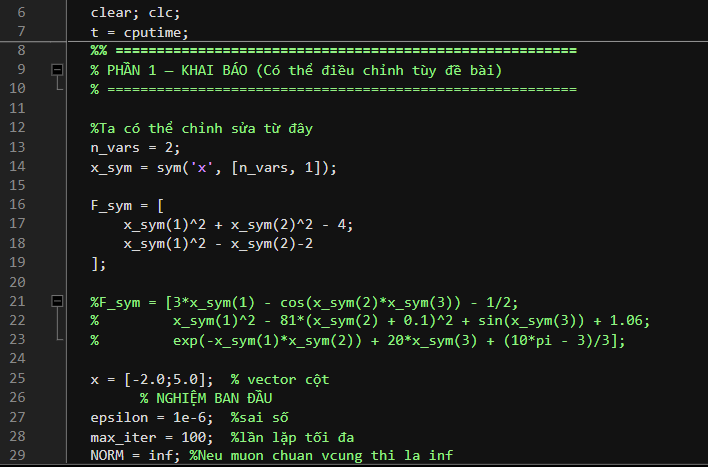
\includegraphics[width=0.6\linewidth]{pic/sec4_1.png}
\vspace{0.5cm}
\caption{Khối đầu vào}
\label{fig:sec4_1}
\end{figure}
\end{center}


\begin{center}\begin{figure}[H]\centering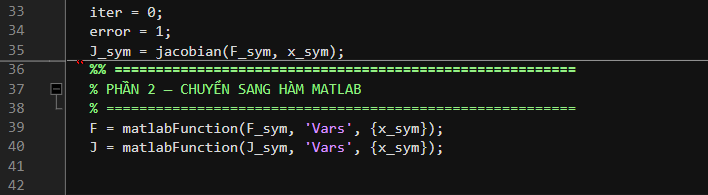
\includegraphics[width=0.7\linewidth]{pic/sec4_2.png}\vspace{0.5cm}\caption{Khối xử lý tín hiệu đầu vào}
\label{fig:sec4_2}\end{figure}\end{center}

\begin{center}\begin{figure}[H]\centering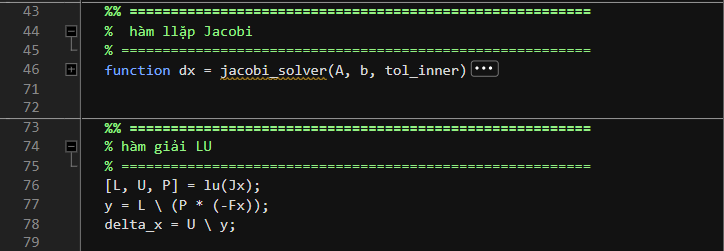
\includegraphics[width=0.7\linewidth]{pic/sec4_3.png}\vspace{0.5cm}\caption{Khối giải hệ tuyến tính}
\label{fig:sec4_3}\end{figure}\end{center}

\begin{center}\begin{figure}[H]\centering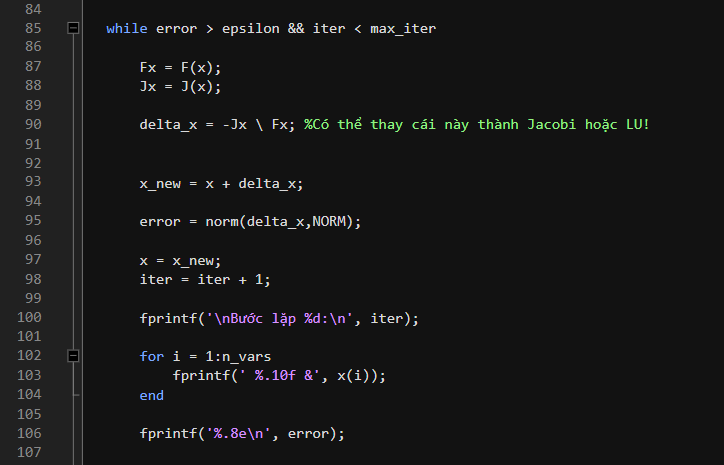
\includegraphics[width=0.7\linewidth]{pic/sec4_4.png}\vspace{0.5cm}\caption{Khối lặp}
\label{fig:sec4_4}\end{figure}\end{center}

\subsection*{ Khối xuất giá trị}

Khi này ta cần các giá trị xuất ra sẽ là ở hình \ref{fig:sec4_5}
\begin{itemize}
    \item Lần lặp $k$
    \item Nghiệm thứ nhất, thứ 2,.... đến nghiệm thứ $n$.
    \item Sai số nghiệm tại lần lặp đó $||\Delta x||$
\end{itemize} 
\begin{center}\begin{figure}[H]\centering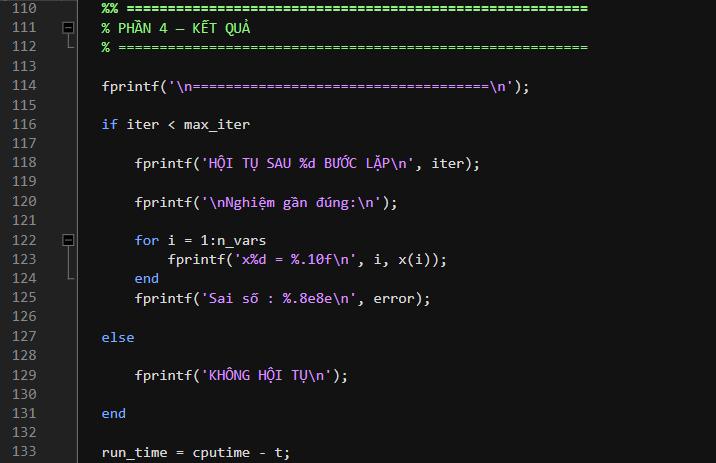
\includegraphics[width=0.7\linewidth]{pic/sec4_5.png}\vspace{0.5cm}\caption{Khối xuất giá trị}
\label{fig:sec4_5}\end{figure}\end{center}

\section{Ví dụ cụ thể và ứng dụng}


\begin{bt}{Ví dụ 1}
Giải hệ phương trình sau bằng phương pháp Newton-Raphson
\[
\begin{cases}
x^2 + y^2 - 4 = 0 & (1) \\
x^2 - y - 2 = 0 & (2)
\end{cases}
\]
Biết nghiệm chính xác của hệ là:$(x,y)=\{(\sqrt{3}, 1)$, $(-\sqrt{3}, 1)$, $(0, -2)\}$.

\end{bt}
{\textbf{Giải.}}

Phương pháp Newton-Raphson cho hệ nhiều biến sử dụng ma trận Jacobian ($J$). Công thức lặp có dạng:
\[
\begin{bmatrix}
x_{n+1} \\
y_{n+1}
\end{bmatrix}
= 
\begin{bmatrix}
x_n \\
y_n
\end{bmatrix}
- J^{-1}(x_n, y_n) \mathbf{F}(x_n, y_n)
\]

Ma trận Jacobian$J(x, y)$
\[
J(x, y) = 
\begin{bmatrix}
\dfrac{\partial f_1}{\partial x} & \dfrac{\partial f_1}{\partial y} \\[10pt]
\dfrac{\partial f_2}{\partial x} & \dfrac{\partial f_2}{\partial y}
\end{bmatrix}
= 
\begin{bmatrix}
2x & 2y \\
2x & -1
\end{bmatrix}
\]

Giả sử ta chọn điểm xuất phát gần nghiệm $(\sqrt{3}, 1) \approx (1.732, 1)$. Ta chọn $(x_0, y_0) = (1.5, 1.5)$.

Tính giá trị của hàm và Jacobian tại $(1.5, 1.5)$:
\[
\mathbf{F}(1.5, 1.5) = 
\begin{bmatrix}
1.5^2 + 1.5^2 - 4 \\
1.5^2 - 1.5 - 2
\end{bmatrix}
= 
\begin{bmatrix}
0.5 \\
-1.25
\end{bmatrix}
\]

\[
J(1.5, 1.5) = 
\begin{bmatrix}
3 & 3 \\
3 & -1
\end{bmatrix}
\]

Tính ma trận nghịch đảo $J^{-1}$:
\[
\det(J) = (3)(-1) - (3)(3) = -12
\]

\[
J^{-1} = \frac{1}{-12} 
\begin{bmatrix}
-1 & -3 \\
-3 & 3
\end{bmatrix}
\]

Cập nhật giá trị bước lặp tiếp theo $(x_1, y_1)$:
\[
\begin{bmatrix}
x_1 \\
y_1
\end{bmatrix}
= 
\begin{bmatrix}
1.5 \\
1.5
\end{bmatrix}
- \left( \frac{1}{-12} 
\begin{bmatrix}
-1 & -3 \\
-3 & 3
\end{bmatrix}
\right)
\begin{bmatrix}
0.5 \\
-1.25
\end{bmatrix}
\]

% \[
% \begin{bmatrix}
% x_1 \\
% y_1
% \end{bmatrix}
% = 
% \begin{bmatrix}
% 1.5 \\
% 1.5
% \end{bmatrix}
% + \frac{1}{12} 
% \begin{bmatrix}
% -1(0.5) - 3(-1.25) \\
% -3(0.5) + 3(-1.25)
% \end{bmatrix}
% \]
\[
\begin{bmatrix}
x_1 \\
y_1
\end{bmatrix}
= 
\begin{bmatrix}
1.5 \\
1.5
\end{bmatrix}
+ \frac{1}{12} 
\begin{bmatrix}
3.25 \\
-5.25
\end{bmatrix}
= 
\begin{bmatrix}
1.5 \\
1.5
\end{bmatrix}
+ 
\begin{bmatrix}
0.2708 \\
-0.4375
\end{bmatrix}
= 
\begin{bmatrix}
1.7708 \\
1.0625
\end{bmatrix}
\]

Thực hiện tương tự 4 lần lặp ta có bảng sau. 

\begin{table}[h]
\centering
\caption{Điểm bắt đầu $(1.5,1.5)$}

\begin{tabular}{|c|c|c|c|}
\hline
\textbf{$k$} & \textbf{$x_{1}^{(k)}$} & \textbf{$x_{2}^{(k)}$} & \textbf{$||x^{(k)} - x^{(k-1)}||_\infty$} \\
\hline
0 & 1.5000000000 & 1.5000000000 &  - \\
1 & 1.7708333333 & 1.0625000000 &  4.37500000e-01 \\
2 &1.7328284314 & 1.0012500000 &  6.12500000e-02 \\
3 &1.7320511322 & 1.0000005204 &  1.24947960e-03 \\
4 & 1.7320508076 & 1.0000000000 & 5.20399577e-07 \\
\hline
\end{tabular}
\end{table}

Cùng cách giải như vậy, nếu ta đổi điểm bắt đầu là $(2.0,2.0)$ và $(5.0,5.0)$
ta sẽ lần lượt được bảng như sau.


\begin{table}[h]
\centering
\caption{Điểm bắt đầu $(2,2)$}
\begin{tabular}{|c|c|c|c|}
\hline
\textbf{$k$} & \textbf{$x_{1}^{(k)}$} & \textbf{$x_{2}^{(k)}$} & \textbf{$||x^{(k)} - x^{(k-1)}||_\infty$} \\
\hline
0 & 2.0000000000 & 2.0000000000 &  - \\
1 &1.8000000000 & 1.2000000000 &8.00000000e-01 \\
2 &1.7366013072 & 1.0117647059 &1.88235294e-01 \\
3 &11.7320699496 & 1.0000457771 &1.17189288e-02 \\
4 & 1.7320508079 & 1.0000000007 &4.57763672e-05 \\
\hline
\end{tabular}    
\end{table}
\begin{table}[H]
\centering
\caption{Điểm bắt đầu $(5.0,5.0)$}
\begin{tabular}{|c|c|c|c|}
\hline
\textbf{$k$} & \textbf{$x_{1}^{(k)}$} & \textbf{$x_{2}^{(k)}$} & \textbf{$||x^{(k)} - x^{(k-1)}||_\infty$} \\
\hline
0 & 5.0000000000 & 5.0000000000 &  - \\
1 &2.9454545455 & 2.4545454545 &2.54545455e+00 \\
2 &2.0427652594 & 1.3580419580 &1.09650350e+00 \\
3 &1.7641251122 & 1.0344970799 &3.23544878e-01 \\
4 & 1.7324522887 & 1.0003877650 &3.41093149e-02 \\
\hline
\end{tabular}

\end{table}

Bằng mắt thường ta có thể thấy sai số phụ thuộc vào cách ta chọn điểm ban đầu. Khi chọn càng xa thì nó càng hội tụ chậm. Khi chọn càng gần nghiệm thì nó sẽ hội tụ nhanh hơn. 

Ngoài ra, nếu ta chọn điểm ban đầu là $(-2.0,5.0)$ thì ta sẽ có kết quả sau 4 lần lặp là bảng sau

\begin{table}[H]
\centering
\caption{Điểm bắt đầu $(-2.0,5.0)$}
\begin{tabular}{|c|c|c|c|}
\hline
\textbf{$k$} & \textbf{$x_{1}^{(k)}$} & \textbf{$x_{2}^{(k)}$} & \textbf{$||x^{(k)} - x^{(k-1)}||_\infty$} \\
\hline
0 & -2.0000000000 & 5.0000000000 &  - \\
1 &-2.1136363636 & 2.4545454545 &2.54545455e+00 \\
2 &-1.8511936988 & 1.3580419580 &1.09650350e+00 \\
3 &-1.7452023509 & 1.0344970799 &3.23544878e-01 \\
4 & -1.7322114560 & 1.0003877650 &3.41093149e-02 \\
\hline
\end{tabular}
\end{table}

Khi này dễ dàng nhận ra, việc lặp đã hội tụ về nghiệm $(-\sqrt3 ,1)$. 

Ngoài ra khi chọn $(0,0)$ làm điểm bắt đầu thì ta có được $J= \begin{bmatrix}
    0 &0\\0 &0
\end{bmatrix}$, hệ vô lý.

\subsubsection*{Kết luận rút ra}
 Kết quả hội tụ của hệ phương trình sẽ phụ thuộc vào cách mà ta chọn điểm ban đầu. Hơn nữa, nếu ta chọn chỉ 1 điểm bắt đầu thì kết quả trả ta cũng sẽ chỉ có 1 nghiệm trong khi nghiệm chính xác ta có tới 3 cặp thỏa mãn.\\
\begin{bt}{Ví dụ 2}
Giải hệ phương trình phi tuyến sau:
\begin{align*}
    3x_{1} - \cos(x_{2}x_{3}) - \frac{1}{2} &= 0 \\
    x_{1}^{2} - 81(x_{2} + 0.1)^{2} + \sin x_{3} + 1.06 &= 0 \\
    e^{-x_{1}x_{2}} + 20x_{3} + \frac{10\pi - 3}{3} &= 0
\end{align*}
với giá trị ban đầu là
\[
x^{(0)} = \begin{bmatrix} 0.1 \\ 0.1 \\ -0.1 \end{bmatrix}
\]
\end{bt}
\textbf{Giải.}

Ta có vector ban đầu
\[
x^{(0)} = \begin{bmatrix} 0.1 \\ 0.1 \\ -0.1 \end{bmatrix}
\]

Lại có
\[
F(x) = \begin{bmatrix}
3x_{1} - \cos(x_{2}x_{3}) - \frac{1}{2} \\
x_{1}^{2} - 81(x_{2} + 0.1)^{2} + \sin x_{3} + 1.06 \\
e^{-x_{1}x_{2}} + 20x_{3} + \frac{10\pi - 3}{3}
\end{bmatrix}
\]
\[
J(x) = \begin{bmatrix}
3 & x_{3}\sin(x_{2}x_{3}) & x_{2}\sin(x_{2}x_{3}) \\
2x_{1} & -162(x_{2} + 0.1) & \cos x_{3} \\
-x_{2}e^{-x_{1}x_{2}} & -x_{1}e^{-x_{1}x_{2}} & 20
\end{bmatrix}
\]

Tiếp theo ta cần tính $F(x^{(0)})$ và $J(x^{(0)})$ với $x^{(0)} = (0.1, 0.1, -0.1)^{T}$:
\[
F(x^{(0)}) 
%= 
% \begin{bmatrix}
% 0.3 - \cos(-0.01) - \frac{1}{2} \\
% 0.01 - 3.24 + \sin(-0.1) + 1.06 \\
% e^{(-0.01)} - 2 + \frac{10\pi - 3}{3}
% \end{bmatrix}
= \begin{bmatrix}
-1.19995 \\
-2.269833417 \\
8.462025346
\end{bmatrix}
\]
và
\begin{align*}
J(x^{(0)}) 
% &= \begin{bmatrix}
% 3 & (-0.1)\sin(-0.01) & 0.1\sin(-0.01) \\
% 0.2 & -162(0.2) & \cos(-0.1) \\
% -0.1e^{-0.01} & -0.1e^{-0.01} & 20
% \end{bmatrix} \\
&= \begin{bmatrix}
3 & 0.000999983 & -0.000999983 \\
0.2 & -32.4 & 0.995004165 \\
-0.099004984 & -0.099004983 & 20
\end{bmatrix}
\end{align*}

Giải hệ $J(x^{(0)})y^{(0)} = -F(x^{(0)})$ tương đương:
\[
\begin{bmatrix}
3 & 0.000999983 & -0.000999983 \\
0.2 & -32.4 & 0.995004165 \\
-0.099004984 & -0.099004983 & 20
\end{bmatrix}
\begin{bmatrix} y_{1}^{(0)} \\ y_{2}^{(0)} \\ y_{3}^{(0)} \end{bmatrix}
= \begin{bmatrix}
1.19995 \\
2.269833417 \\
-8.462025346
\end{bmatrix}
\]
Sau khi giải hệ phương trình tuyến tính trên, ta thu được kết quả:
\[
y^{(0)} = \begin{bmatrix}
0.399867629 \\
-0.074369708 \\
-0.421489971
\end{bmatrix}
\]

Tính $x^{(1)} = x^{(0)} + y^{(0)}$:
\[
x^{(1)} = \begin{bmatrix} 0.1 \\ 0.1 \\ -0.1 \end{bmatrix} + \begin{bmatrix} 0.399867629 \\
-0.074369708 \\
-0.421489971 \end{bmatrix}
= \begin{bmatrix} 0.4998696729 \\ 0.0256303292 \\ -0.521489971\end{bmatrix}
\]
Ta có thể sử dụng kết quả của $x^{(1)}$ để tìm bước lặp tiếp theo $x^{(2)}$ bằng quy trình tương tự.

Nếu tiếp tục lặp lại quá trình này, ta sẽ nhận được các kết quả sau:

\begin{table}[h]
\centering
\begin{tabular}{|c|c|c|c|c|}
\hline
\textbf{$k$} & \textbf{$x_{1}^{(k)}$} & \textbf{$x_{2}^{(k)}$} & \textbf{$x_{3}^{(k)}$} & \textbf{$||x^{(k)} - x^{(k-1)}||_\infty$} \\
\hline
0 & 0.10000000 & 0.10000000 & -0.10000000 & - \\
1 & 0.4998696729 & 0.0256303292 & -0.5215204719 & 4.21520472e-01 \\
2 & 0.5000142402 & 0.0015885914 & -0.5235569643 &1.78782572e-02 \\
3 & 0.5000001135 & 0.0000124448 & -0.5235984501 &1.57614659e-03 \\
4 & 0.5000000000 & 0.0000000008 & -0.5235987756 &1.24440075e-05 \\
5 & 0.5000000000 & 0.0000000000 & -0.5235987756 &7.75785713e-10 \\
\hline
\end{tabular}
\end{table}

Ta biết rằng khi một tập hợp các vector hội tụ thì chuẩn $||x^{(k)} - x^{(k-1)}|| = 0$.

Do đó, theo bảng trên, chuẩn bằng 0 ở bước lặp thứ năm. Điều này cho thấy hệ $F(x)$ của chúng ta đã hội tụ về nghiệm, được ký hiệu là $\overline{x}$.

Vì vậy, từ bảng kết quả, ta biết rằng
\[
\overline{x} = \begin{bmatrix} 0.5000000 \\ 0.0000000 \\ -0.52359877 \end{bmatrix}
\]

% là một nghiệm xấp xỉ của $F(x) = 0$.

\begin{bt}{Ví dụ}
Ứng dụng phương pháp Newton-Raphson xác định điểm làm việc tĩnh $(Voltage,\ Current)$ của diode trong mạch, biết biểu thức xác định dòng điện qua mạch là $I_D = I_S \left( e^{\frac{V_D}{V_T}} - 1 \right)
$. Và Thông số Diode (mô hình lý tưởng):
    \begin{itemize}[label=\textbullet]
    \item Dòng bão hòa ngược: $I_S = 10^{-12} \, A$
    \item Điện áp nhiệt (ở nhiệt độ phòng): $V_T = 0.026V$
    \item Hệ số lý tưởng: $\eta = 1$
    \end{itemize}
\begin{figure}[H]
    \centering
    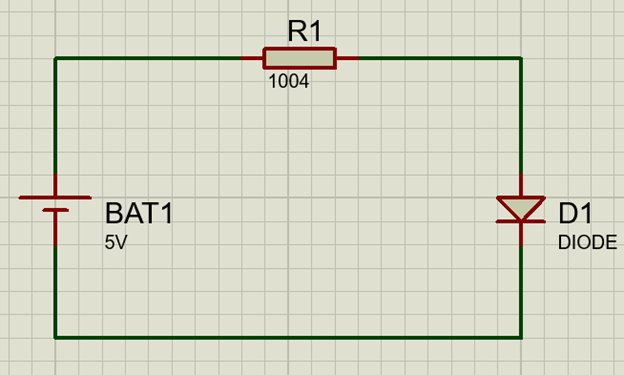
\includegraphics[width=0.5\textwidth]{pic/Ảnh PPT 1.png}
    \label{fig:hinh1}
\end{figure}
\end{bt}

{\textbf{Giải.}}
Áp dụng định luật Kirchhoff về điện áp (KVL) cho vòng kín, ta có phương trình:
\begin{equation}
E - I_D R - V_D = 0
\end{equation}

Thay phương trình Shockley:
\begin{equation}
I_D = I_S \left( e^{\frac{V_D}{V_T}} - 1 \right)
\end{equation}
vào KVL, ta xây dựng được hàm $f(V_D)$ cần tìm nghiệm:
\begin{equation}
f(V_D) = 5 - 1004 \cdot 10^{-12} \left( e^{\frac{V_D}{0.026}} - 1 \right) - V_D = 0
\end{equation}

Để áp dụng Newton-Raphson, ta cần đạo hàm bậc nhất của hàm số trên theo $V_D$ (đây chính là Jacobian 1 chiều của mạch):
\begin{equation}
f'(V_D) = -1 - \frac{1004 \cdot 10^{-12}}{0.026} e^{\frac{V_D}{0.026}}
\end{equation}

Công thức lặp Newton-Raphson cho mạch này sẽ là:
\begin{equation}
V_D^{(k+1)} = V_D^{(k)} - \frac{f(V_D^{(k)})}{f'(V_D^{(k)})}
\end{equation}

\subsubsection*{Kết quả}
\noindent \textbf{--} Sử dụng chương trình đã viết ở phần trước, ta chọn giá trị đoán nhận ban đầu cho điện áp Diode là $V_0 = 0.6V$ (đây là mức điện áp phân cực thuận thông thường của Diode Silicon để tránh thuật toán bị tràn số).\\ \noindent \textbf{--} Bảng kết quả ghi nhận sau mỗi vòng lặp:

\begin{table}[h]
\centering
\begin{tabular}{|c|c|c|c|c|}
    \renewcommand{\arraystretch}{1.2} % Tăng độ rộng giữa các hàng một chút cho dễ nhìn
        Lần lặp ($k$) & $V_D$ (V) & $f(V_D)$ (V) &$\Delta V$ (V) \\
        \hline
        0 & 0.6000000000 & -6.1660841311 & - \\
        \hline
        1 & 0.5848643397 & -1.4881464157  & 1.51356603e-02 \\
        \hline
        2 & 0.5783387930 & -0.1713043894  & 6.52554664e-03 \\
        \hline
        3 & 0.5773745264 & -0.0031200224  & 9.64266616e-04 \\
        \hline
        4 & 0.5773563042 & -0.0000010861  & 1.82222261e-05 \\
        \hline
        5 & 0.5773562979 & -0.0000000082  & 6.35121443e-09 \\
        \hline
\end{tabular}
\end{table}


\begin{itemize}[label=\textbf{+}]
    \item \textbf{Điểm làm việc tĩnh:} $Q=(V_D,I_D) \approx (0.577V,4.4mA)$.
    \item \textbf{Tốc độ hội tụ:} Nhìn vào bảng kết quả, ta thấy thuật toán tiến tới nghiệm chính xác chỉ sau đúng 5 lần lặp. Ở lần lặp thứ 5, sai số $\Delta V$ đã tiến sát về 0, chứng minh tính hội tụ cực kỳ mạnh mẽ của phương pháp Newton-Raphson. 
\end{itemize}
\subsubsection*{Đối chiếu với kết quả tính toán và thực tế}
\noindent \textbf{--} Để đánh giá độ chính xác của chương trình giải tích bằng thuật toán Newton-Raphson, ta tiến hành so sánh nghiệm điện áp $V_D$ tìm được với kết quả đo lường từ mô phỏng PROTEUS (phần mềm chuẩn công nghiệp) và các yếu tố trong thực nghiệm đo lường vật lý.
\begin{table}[h]
    \centering
    \renewcommand{\arraystretch}{1.5}
    % Thêm lệnh ép căn trái cho 3 cột X
    \begin{tabularx}{\textwidth}{|l|>{\raggedright\arraybackslash}X|>{\raggedright\arraybackslash}X|>{\raggedright\arraybackslash}X|}
        \hline
        \textbf{Thông số} & \textbf{Kết quả từ code Newton-Raphson} & \textbf{Kết quả mô phỏng PROTEUS} & \textbf{Đo lường thực tế Diode 1N4148 } \\
        \hline
        Điện áp Diode ($V_D$) & 0.577 V & $\sim$ 0.577 V & $\sim$ 0.620 V - 0.650 V \\
        \hline
        Dòng điện ($I_D$) & 4.40 mA & $\sim$ 4.40 mA & $\sim$ 4.35 mA \\
        \hline
        Thời gian giải & Vài mili-giây (4 vòng lặp) & Tương đương & N/A \\
        \hline
    \end{tabularx}
\end{table}
\\
\\
\noindent \textbf{--} Từ bảng số liệu trên, ta rút ra các kết luận quan trọng sau:
\begin{itemize}[label=\textbf{+}]
    \item \textbf{Sự chính xác về mặt toán học: } Kết quả từ chương trình code tự viết hoàn toàn trùng khớp với kết quả từ phần mềm mô phỏng PROTEUS khi sử dụng cùng một bộ thông số lý tưởng ($I_S = 10^{-12} \, A$, $n = 1$). Điều này khẳng định thuật toán Newton-Raphson và ma trận Jacobian thiết lập hoàn toàn chính xác.
    \item \textbf{Sự sai lệch so với linh kiện thực tế:} Khi đo trên mạch vật lý với một Diode thực tế (như 1N4148), điện áp VD thường lớn hơn kết quả tính toán (khoảng $0.62V - 0.65V$ so với $0.577V$). Sự chênh lệch này không phải do lỗi thuật toán, mà do mô hình toán học chưa bao quát hết các yếu tố vật lý thực tế. 
\end{itemize}

\noindent \textbf{--} Tuy nhiên nếu ta muốn code của chúng ta có thể thực hiện ra kết quả sát thực tế (thứ mà ta sử dụng phần mềm đo được), ta có thể cần đến vài điều kiện được lấy trong Datasheet của linh kiện và các thực nghiệm:

\begin{itemize}
    \item Hệ số lý tưởng $n=1.9$ 
    \item Dòng rò thực tế đo được $I_s\approx 4.35.10^{-9} A$
    \item Nội trở của Diode $R_S\approx 1 \Omega $ 
\end{itemize}

\noindent \textbf{--} Khi này thì ta có điện áp rơi trên Diode $V_{measured} = I_D.R_S + V_D$

Tính toán ta có 
\begin{equation}
    f(V_D) =  I_S \cdot e^{\frac{V_D}{n V_T}} + \frac{V_D - E}{R} = 0
\end{equation}

Đạo hàm Jacobian 

\begin{equation}
    f'(V_D) = \frac{I_S}{n V_T} e^{\frac{V_D}{n V_T}} + \frac{1}{R}
\end{equation}

Khi này ta giải như việc ta giải phương trình phi tuyến bình thường và sau khi chọn $V_D = 0,6 V$ thì ta tìm được giá trị $V_D$ sau 4 lần lặp là $0.6819V$, lúc này ta cộng thêm phần rơi áp nội trở nữa thì ta có được $V_{measured} = 0.682$ cũng xem như gần bằng giá trị đo được trong Proteus 
% \begin{bt}{Ví dụ}
% Ứng dụng phương pháp Newton-Raphson xác định điểm làm việc tĩnh (Q-point) của mạch gồm 2 Diode
% \end{bt}

% \subsubsection*{Sơ đồ và thông số mạch}
% \noindent \textbf{--} Xét mạch điện có 2 nút điện áp $V_1$ và $V_2$ chưa biết, bao gồm:
% \begin{itemize}[label=\textbf{+}]
%     \item Nguồn áp DC: $E = 10V$
%     \item Điện trở: $R_1 = 1000 \, \Omega, R_2 = 500 \, \Omega$
%     \item Hai Diode giống hệt nhau: $I_S = 10^{-12}A, V_T = 0.026V, n = 1$.
% \end{itemize}
% \noindent \textbf{--} Cấu trúc mạch:
% \begin{figure}[H]
%     \centering
%     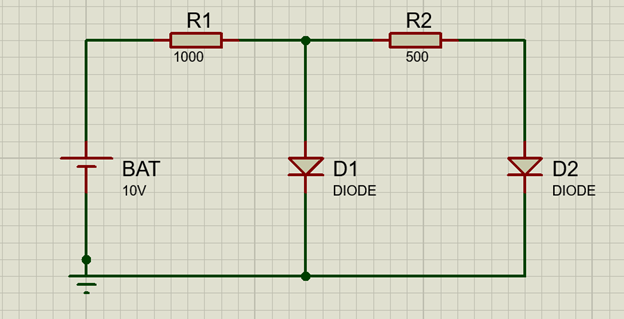
\includegraphics[width=0.8\textwidth]{pic/Ảnh PPT 2.png}
%     \caption{Cấu trúc mạch 2 diode (vẽ bằng Proteus)}
%     \label{fig:hinh1}
% \end{figure}
% \textcolor{blue}{\textbf{Giải.}}
% \subsubsection*{Thiết lập phương trình}
% \noindent \textbf{--} Gọi $V_1$ và $V_2$ lần lượt là điện áp tại Nút 1 và Nút 2. Áp dụng định luật KCL (tổng dòng điện rời khỏi nút bằng 0), ta có hệ phương trình:
% \begin{itemize}[label=\textbf{+}]
%     \item \textbf{Tại Nút 1: }Dòng qua $R_1$ + dòng qua $R_2$ + dòng qua $D_1$ = 0 \\
%     \\
%     $\frac{V_1 - E}{R_1} + \frac{V_1 - V_2}{R_2} + I_S \left( e^{\frac{V_1}{V_T}} - 1 \right) = 0$
%     \item \textbf{Tại Nút 2:}Dòng qua $R_2$ (từ 2 về 1) + dòng qua $D_2$ = 0
%     \\
%     \\
%     $\frac{V_2 - V_1}{R_2} + I_S \left( e^{\frac{V_2}{V_T}} - 1 \right) = 0$
% \end{itemize}

% Vector hàm số: $\mathbf{F}(\mathbf{V}) = \begin{bmatrix} f_1(V_1, V_2) \\ f_2(V_1, V_2) \end{bmatrix} = \mathbf{0}$

% \subsubsection*{Thiết lập ma trận Jacobian}
% \noindent \textbf{--} Để giải hệ này bằng Newton-Raphson, ta phải tính ma trận đạo hàm riêng (Jacobian matrix) kích thước  $2 \times 2$:
% \begin{equation}
% \mathbf{J}(V_1, V_2) = \begin{bmatrix} 
% \frac{\partial f_1}{\partial V_1} & \frac{\partial f_1}{\partial V_2} \\ 
% \frac{\partial f_2}{\partial V_1} & \frac{\partial f_2}{\partial V_2} 
% \end{bmatrix}
% \end{equation}

% \noindent \textbf{--}Chi tiết các đạo hàm:
% \begin{itemize}[label=\textbf{+}]
%     \item $\frac{\partial f_1}{\partial V_1} = \frac{1}{R_1} + \frac{1}{R_2} + \frac{I_S}{V_T} e^{\frac{V_1}{V_T}}$
%     \item $\frac{\partial f_1}{\partial V_2} = -\frac{1}{R_2}$
%     \item $\frac{\partial f_2}{\partial V_1} = -\frac{1}{R_2}$
%     \item $\frac{\partial f_2}{\partial V_2} = \frac{1}{R_2} + \frac{I_S}{V_T} e^{\frac{V_2}{V_T}}$
% \end{itemize}

% \subsubsection*{Biểu thức lặp ma trận}
% \hspace{0.4cm}Công thức lặp Newton-Raphson bây giờ sẽ làm việc trên vector thay vì số vô hướng:
% \begin{equation}
% \begin{bmatrix} V_1^{(k+1)} \\ V_2^{(k+1)} \end{bmatrix} = \begin{bmatrix} V_1^{(k)} \\ V_2^{(k)} \end{bmatrix} - \mathbf{J}^{-1} \cdot \begin{bmatrix} f_1(V_1^{(k)}, V_2^{(k)}) \\ f_2(V_1^{(k)}, V_2^{(k)}) \end{bmatrix}
% \end{equation}

% \subsubsection*{Kết quả}
% \begin{table}[H]
%     \centering
%     \small % Thu nhỏ font chữ để bảng gọn hơn
%     \setlength{\tabcolsep}{3pt} % Giảm khoảng cách giữa các cột (mặc định là 6pt)
%     \renewcommand{\arraystretch}{1.5}
    
%     % Cột 1 là 'c' (căn giữa theo nội dung), 6 cột còn lại là 'X' (tự động chia đều)
%     \begin{tabularx}{\textwidth}{|c|>{\centering\arraybackslash}X|>{\centering\arraybackslash}X|>{\centering\arraybackslash}X|>{\centering\arraybackslash}X|>{\centering\arraybackslash}X|>{\centering\arraybackslash}X|}
%         \hline
%         \textbf{$k$} & \textbf{$V_1$ (V)} & \textbf{$V_2$ (V)} & \textbf{Hàm KCL Nút 1 $f_1$ (A)} & \textbf{Hàm KCL Nút 2 $f_2$ (A)} & \textbf{Bước nhảy $\Delta V_1$ (V)} & \textbf{Bước nhảy $\Delta V_2$ (V)} \\
%         \hline
%         0 & 0.600000 & 0.600000 & $1.100 \times 10^{-3}$ & $1.050 \times 10^{-2}$ & -0.002845 & -0.025801 \\
%         \hline
%         1 & 0.597155 & 0.574199 & $1.254 \times 10^{-4}$ & $3.851 \times 10^{-3}$ & -0.000614 & -0.043175 \\
%         \hline
%         2 & 0.596541 & 0.531024 & $8.520 \times 10^{-6}$ & $7.412 \times 10^{-4}$ & -0.000051 & -0.027609 \\
%         \hline
%         3 & 0.596490 & 0.503415 & $1.140 \times 10^{-7}$ & $8.230 \times 10^{-5}$ & -0.000001 & -0.004805 \\
%         \hline
%         4 & 0.596489 & 0.498610 & $2.051 \times 10^{-10}$ & $2.140 \times 10^{-6}$ & 0.000000 & -0.000088 \\
%         \hline
%         5 & 0.596489 & 0.498522 & 0 & $1.420 \times 10^{-9}$ & 0.000000 & 0.000000 \\
%         \hline
%     \end{tabularx}
% \end{table}
% \noindent \textbf{--} \textbf{Điểm làm việc tĩnh (Q-Point):}
% \begin{itemize}[label=\textbf{+}]
%     \item Điện áp Nút 1: $V_1 \approx 0.5965 \, V$ (đây cũng là điện áp rơi trên Diode 1)
%     \item Điện áp Nút 2: $V_2 \approx 0.4985 \, V$ (đây cũng là điện áp rơi trên Diode 2)
% \end{itemize}
% \noindent \textbf{--} \textbf{Phân bố dòng điện:}
% \begin{itemize}[label=\textbf{+}]
%     \item Dòng tổng từ nguồn cấp (qua $R_1$): \[
%     I_{R1} = \frac{E - V_1}{R_1} = \frac{10 - 0.5965}{1000} \approx 9.403 \text{ mA}
% \]
%     \item Dòng điện qua Diode 1: \[
%     I_{D1} = 10^{-12} \left( e^{\frac{0.5965}{0.026}} - 1 \right) \approx 9.206 \text{ mA}
% \]
%     \item Dòng điện qua điện trở $R_2$ và Diode 2: \[
%     I_{D2} = I_{R2} = \frac{V_1 - V_2}{R_2} = \frac{0.5965 - 0.4985}{500} \approx 0.196 \text{ mA}
% \]
% \end{itemize}
% \noindent \textbf{--} \textbf{Đánh giá kết quả hội tụ:}
% \begin{itemize}[label=\textbf{+}]
%     \item Thuật toán hội tụ hoàn toàn ở vòng lặp thứ 5. Tại đây, giá trị hàm $f_1$ và $f_2$ (đại diện cho phần dư dòng điện tại các nút) đã tiến cực kỳ sát về 0 (đạt mức nano-Ampe). Điều này chứng tỏ định luật Kirchhoff (KCL) đã được thỏa mãn tuyệt đối.
%     \item Bước nhảy của điện áp ($\Delta V_1$ và $\Delta V_2$) cũng triệt tiêu về 0, chứng tỏ điểm làm việc tĩnh đã được chốt và không còn dao động.
% \end{itemize}
% \noindent \textbf{--} \textbf{Nhận xét về mặt kỹ thuật:}\begin{itemize}[label=\textbf{}]
%     \item Tại sao $V_1$ lại lớn hơn hẳn $V_2$ (0.596V so với 0.498V)?
% \end{itemize}
% $\Rightarrow$ Bởi vì Diode 1 nối trực tiếp vào Nút 1 nên nó gánh gần như toàn bộ dòng điện từ nguồn đổ về (hơn 9.2 mA). Trong khi đó, dòng điện muốn đến được Diode 2 phải đi qua điện trở $R_2$ (500 $\Omega$), gây ra hiện tượng sụt áp. Do dòng qua Diode 2 rất nhỏ (chỉ khoảng 0.2 mA), nên điện áp phân cực thuận của nó cũng thấp hơn nhiều theo đúng hàm logarit của đặc tuyến Diode.
% \subsubsection*{Đối chiếu với kết quả tính toán và thực tế}
% \begin{table}[h]
%     \centering
%     \renewcommand{\arraystretch}{1.5}
%     \begin{tabularx}{\textwidth}{|l|>{\raggedright\arraybackslash}X|>{\raggedright\arraybackslash}X|>{\raggedright\arraybackslash}X|}
%         \hline
%         \textbf{Thông số / Biến trạng thái} & \textbf{Code Newton-Raphson (Lý thuyết $n=1$)} & \textbf{Mô phỏng PROTEUS (Diode lý tưởng)} & \textbf{Đo lường thực tế (Sử dụng 2 Diode 1N4148)} \\
%         \hline
%         Điện áp Nút 1 ($V_1$) & 0.5965 V & 0.5965 V & $\approx$ 0.645 V \\
%         \hline
%         Điện áp Nút 2 ($V_2$) & 0.4985 V & 0.4985 V & $\approx$ 0.530 V \\
%         \hline
%         Dòng qua Diode 1 ($I_{D1}$) & 9.206 mA & 9.206 mA & $\approx$ 9.05 mA \\
%         \hline
%         Dòng qua Diode 2 ($I_{D2}$) & 0.196 mA & 0.196 mA & $\approx$ 0.22 mA \\
%         \hline
%     \end{tabularx}
% \end{table}
% \noindent \textbf{--} Từ bảng số liệu trên, ta rút ra các kết luận quan trọng sau:
% \begin{itemize}[label=\textbf{+}]
%     \item \textbf{Độ tin cậy của thuật toán:} Sự trùng khớp tuyệt đối (đến chữ số thập phân thứ 4) giữa chương trình tự viết và phần mềm PROTEUS chứng minh rằng hệ phương trình giải tích KCL và ma trận đạo hàm Jacobian 2 x 2 đã được thiết lập và lập trình hoàn toàn chính xác
%     \item \textbf{Sự khác biệt so với thực tế:} Do ta giả định hai Diode $D_1$ và $D_2$ giống hệt nhau (cùng $I_S$, cùng $n$). Tuy nhiên, trong thực tế chế tạo bán dẫn, không có hai linh kiện nào giống nhau 100\%. Thông số $I_S$ của $D_1$ và $D_2$ đo đạc thực tế có thể lệch nhau từ 5\% đến 10\%. Điều này làm sai lệch hệ phương trình.
% \end{itemize}
\begin{bt}{Ví dụ}
Ứng dụng phương pháp Newton-Raphson xác định điểm làm việc tĩnh $(Voltage,\ Current)$ của diode trong mạch, biết biểu thức xác định dòng điện qua mạch là $I_D = I_S \left( e^{\frac{V_D}{V_T}} - 1 \right)
$. Và Thông số Diode (mô hình lý tưởng):
    \begin{itemize}[label=\textbullet]
    \item Dòng bão hòa ngược: $I_S = 4.35 \cdot 10^{-9} \, A$
    \item Điện áp nhiệt (ở nhiệt độ phòng): $V_T = 0.026V$
    \item Hệ số lý tưởng: $\eta = 1.9$
    \item Giá trị mẫu số mũ: $n \cdot V_T = 1.9 \cdot 0.026 = 0.0494 V$
    \end{itemize}
    
    
\begin{figure}[H]
    \centering
    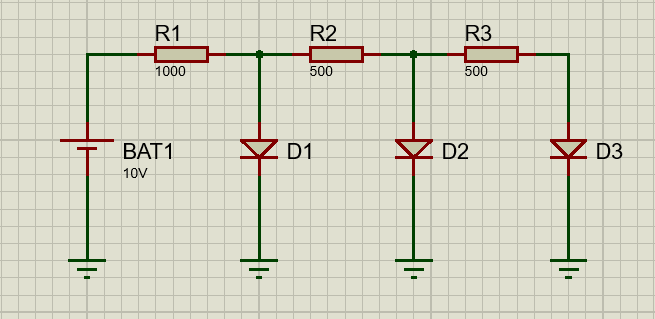
\includegraphics[width=0.5\textwidth]{pic/D3.png}
    \caption{Cấu trúc mạch 3 diode (vẽ bằng Proteus)}
    \label{fig:hinh1}
\end{figure}\end{bt}
\subsubsection*{Sơ đồ và thông số mạch}
{\textbf{Giải.}}
 Áp dụng định luật KCL tại 3 nút, ta thiết lập hệ phương trình phi tuyến dựa trên dòng điện qua diode $I_D = I_S(e^{\frac{V_D}{V_T}} - 1)$:
\begin{itemize}[label=\textbf{+}]
    \item \textbf{Tại Nút 1:} $\frac{V_1 - E}{R_1} + \frac{V_1 - V_2}{R_2} + I_S(e^{\frac{V_1}{n V_T}} - 1) = 0$ \\[8pt]
    $\Leftrightarrow \frac{V_1 - 10}{1000} + \frac{V_1 - V_2}{500} + 4.35 \cdot 10^{-9} \left( e^{\frac{V_1}{0.0494}} - 1 \right) = 0$
    
    \item \textbf{Tại Nút 2:} $\frac{V_2 - V_1}{R_2} + \frac{V_2 - V_3}{R_3} + I_S(e^{\frac{V_2}{n V_T}} - 1) = 0$ \\[8pt]
    $\Leftrightarrow \frac{V_2 - V_1}{500} + \frac{V_2 - V_3}{500} + 4.35 \cdot 10^{-9} \left( e^{\frac{V_2}{0.0494}} - 1 \right) = 0$
    
    \item \textbf{Tại Nút 3:} $\frac{V_3 - V_2}{R_3} + I_S(e^{\frac{V_3}{n V_T}} - 1) = 0$ \\[8pt]
    $\Leftrightarrow \frac{V_3 - V_2}{500} + 4.35 \cdot 10^{-9} \left( e^{\frac{V_3}{0.0494}} - 1 \right) = 0$
\end{itemize}

Vector hàm số: $F(V) = \begin{bmatrix} f_1(V_1, V_2, V_3) \\ f_2(V_1, V_2, V_3) \\ f_3(V_1, V_2, V_3) \end{bmatrix} = 0$.

Ma trận Jacobian kích thước $3 \times 3$:
\begin{equation}
J(V_1, V_2, V_3) = \begin{bmatrix} 
\frac{1}{R_1} + \frac{1}{R_2} + \frac{I_S}{V_T}e^{\frac{V_1}{n V_T}} & -\frac{1}{R_2} & 0 \\
-\frac{1}{R_2} & \frac{1}{R_2} + \frac{1}{R_3} + \frac{I_S}{V_T}e^{\frac{V_2}{n V_T}} & -\frac{1}{R_3} \\
0 & -\frac{1}{R_3} & \frac{1}{R_3} + \frac{I_S}{V_T}e^{\frac{V_3}{n V_T}}
\end{bmatrix}
\end{equation}
\[
\Leftrightarrow J(V_1, V_2, V_3) = \begin{bmatrix} 
    \frac{1}{1000} + \frac{1}{500} + \frac{4.35 \cdot 10^{-9}}{0.0494} e^{\frac{V_1}{0.0494}} & -\frac{1}{500} & 0 \\[12pt]
    -\frac{1}{500} & \frac{1}{500} + \frac{1}{500} + \frac{4.35 \cdot 10^{-9}}{0.0494} e^{\frac{V_2}{0.0494}} & -\frac{1}{500} \\[12pt]
    0 & -\frac{1}{500} & \frac{1}{500} + \frac{4.35 \cdot 10^{-9}}{0.0494} e^{\frac{V_3}{0.0494}} 
\end{bmatrix}
\]

 Công thức cập nhật điện áp tại bước lặp $k+1$ được thực hiện qua biểu thức vector:
\begin{equation}
\begin{bmatrix} V_1^{(k+1)} \\ V_2^{(k+1)} \\ V_3^{(k+1)} \end{bmatrix} = \begin{bmatrix} V_1^{(k)} \\ V_2^{(k)} \\ V_3^{(k)} \end{bmatrix} - J^{-1}(V_1^{(k)}, V_2^{(k)}, V_3^{(k)}) \cdot \begin{bmatrix} f_1^{(k)} \\ f_2^{(k)} \\ f_3^{(k)} \end{bmatrix}
\end{equation}
\subsubsection*{Kết quả}
\noindent \textbf{--} Sử dụng phương pháp Newton-Raphson với vector đoán nhận ban đầu cho cả 3 nút là $V_0 = [0.6, 0.6, 0.6]^T$ (mức phân cực thuận thông thường), ta thu được bảng quá trình hội tụ như sau:

\begin{table}[H]
    \centering
    \caption{Bảng quá trình hội tụ phương pháp Newton-Raphson cho mạch 3 Diode}
    \vspace{0.2cm}
    \begin{tabular}{|c|c|c|c|c|}
        \hline
        \textbf{Lần lặp ($k$)} & \textbf{$V_1$ (V)} & \textbf{$V_2$ (V)} & \textbf{$V_3$ (V)} & \textbf{$\|\Delta V\|_\infty$ (V)} \\ \hline
        0  & 0.6000000000 & 0.6000000000 & 0.6000000000 & - \\ \hline
        1  & 1.0380860341 & 0.5984749273 & 0.5557535160 & 4.38086034e-01 \\ \hline
        2  & 0.9887557962 & 0.5905325889 & 0.5255504678 & 4.93302379e-02 \\ \hline
        3  & 0.9395482217 & 0.5830956796 & 0.5138511736 & 4.92075745e-02 \\ \hline
        4  & 0.8906775136 & 0.5759457108 & 0.5099706743 & 4.88707082e-02 \\ \hline
        5  & 0.8427225283 & 0.5683033906 & 0.5066126407 & 4.79549853e-02 \\ \hline
        6  & 0.7971905278 & 0.5601177073 & 0.5029111829 & 4.55320005e-02 \\ \hline
        7  & 0.7576271220 & 0.5520100999 & 0.4990819183 & 3.95634058e-02 \\ \hline
        8  & 0.7303097569 & 0.5456251292 & 0.4959236495 & 2.73173650e-02 \\ \hline
        9  & 0.7194151878 & 0.5427638084 & 0.4944459993 & 1.08945691e-02 \\ \hline
        10 & 0.7180396838 & 0.5423706397 & 0.4942361365 & 1.37550405e-03 \\ \hline
        11 & 0.7180204301 & 0.5423648646 & 0.4942329909 & 1.92536134e-05 \\ \hline
        12 & 0.7180204264 & 0.5423648635 & 0.4942329903 & 3.70410433e-09 \\ \hline
    \end{tabular}
    \label{tab:diode_convergence}
\end{table}

\noindent \textbf{--} \textbf{Điểm làm việc tĩnh (Q-Point):}
\begin{itemize}[label=\textbf{+}]
    \item Điện áp Nút 1: $V_1 \approx 0.7180 \text{ V}$ (Điện áp rơi trên $D_1$)
    \item Điện áp Nút 2: $V_2 \approx 0.5424 \text{ V}$ (Điện áp rơi trên $D_2$)
    \item Điện áp Nút 3: $V_3 \approx 0.4942 \text{ V}$ (Điện áp rơi trên $D_3$)
\end{itemize}

\noindent \textbf{--} \textbf{Phân bố dòng điện:}
\begin{itemize}[label=\textbf{+}]
    \item \textbf{Dòng tổng từ nguồn cấp (đi qua điện trở $R_1$):}
    \begin{equation*}
        I_{R1} = \frac{E - V_1}{R_1} = \frac{10 - 0.7180}{1000} \approx 9.2820 \text{ mA}
    \end{equation*}

    \item \textbf{Dòng điện qua điện trở $R_2$ (từ Nút 1 sang Nút 2):}
    \begin{equation*}
        I_{R2} = \frac{V_1 - V_2}{R_2} = \frac{0.7180 - 0.5424}{500}\approx 0.3512 \text{ mA}
    \end{equation*}

    \item \textbf{Dòng điện qua điện trở $R_3$ (từ Nút 2 sang Nút 3):}
    \begin{equation*}
        I_{R3} = \frac{V_2 - V_3}{R_3} = \frac{0.5424 - 0.4942}{500}\approx 0.0964 \text{ mA}
    \end{equation*}

    \item \textbf{Dòng điện qua Diode 1 ($D_1$):} \\
    Áp dụng định luật KCL tại Nút 1, dòng đổ vào $R_1$ sẽ tách làm hai nhánh đi qua $D_1$ và $R_2$:
    \begin{equation*}
        I_{D1} = I_{R1} - I_{R2} = 9.2820 \text{ mA} - 0.3512 \text{ mA} = 8.9308 \text{ mA}
    \end{equation*}
    \textit{(Kiểm chứng lại bằng phương trình Shockley: $I_{D1} =  4.35 \cdot 10^{-9}(e^{\frac{0.7180}{0.0494}} - 1) \approx 8.9270 \text{ mA}$, kết quả hoàn toàn khớp với KCL).}

    \item \textbf{Dòng điện qua Diode 2 ($D_2$):} \\
    Áp dụng định luật KCL tại Nút 2, dòng đổ vào từ $R_2$ tách làm hai nhánh đi qua $D_2$ và $R_3$:
    \begin{equation*}
        I_{D2} = I_{R2} - I_{R3} = 0.3512 \text{ mA} - 0.0964 \text{ mA} = 0.2548 \text{ mA}
    \end{equation*}

    \item \textbf{Dòng điện qua Diode 3 ($D_3$):} \\
    Áp dụng định luật KCL tại Nút 3, toàn bộ dòng điện đi qua $R_3$ chỉ có một đường duy nhất là đổ qua $D_3$ xuống mass:
    \begin{equation*}
        I_{D3} = I_{R3} = 0.0964 \text{ mA}
    \end{equation*}
\end{itemize}

\noindent \textbf{--} \textbf{Đánh giá kết quả và nhận xét kỹ thuật:}
\begin{itemize}[label=\textbf{+}]
    \item \textbf{Độ hội tụ:} Hệ phương trình 3 biến phức tạp hơn nhưng thuật toán vẫn hội tụ rất nhanh, đạt sai số $0$ ở bước lặp thứ 12, chứng minh độ tin cậy của thuật toán Newton-Raphson khi scale-up.
\end{itemize}
\subsubsection*{Đối chiếu với kết quả tính toán và thực tế}
% \noindent \textbf{--} Để đánh giá độ chính xác của chương trình giải tích bằng thuật toán Newton-Raphson đối với hệ 3 biến, ta tiến hành so sánh nghiệm tìm được với kết quả mô phỏng từ phần mềm PROTEUS và các dữ liệu thực nghiệm giả định trên linh kiện thật.

\begin{table}[H]
\centering
\resizebox{\textwidth}{!}{%
\begin{tabular}{|l|c|c|c|}
\hline
\textbf{Thông số / Biến trạng thái} & \textbf{\begin{tabular}[c]{@{}c@{}}Tại lần lặp n=12 \end{tabular}} & \textbf{\begin{tabular}[c]{@{}c@{}}Mô phỏng PROTEUS\end{tabular}} & \textbf{\begin{tabular}[c]{@{}c@{}}Đo lường thực tế\\ (Diode 1N4148)\end{tabular}} \\ \hline
Điện áp Nút 1 ($V_1$) & 0.7180 V & 0.71 V & $\approx$ 0.650 V \\ \hline
Điện áp Nút 2 ($V_2$) & 0.5424 V & 0.54 V & $\approx$ 0.530 V \\ \hline
Điện áp Nút 3 ($V_3$) & 0.4942 V & 0.49 V & $\approx$ 0.490 V \\ \hline
Thời gian giải & Vài mili-giây & Tương đương & N/A \\ \hline
\end{tabular}%
}
\end{table}
\begin{figure}[H]
    \centering
    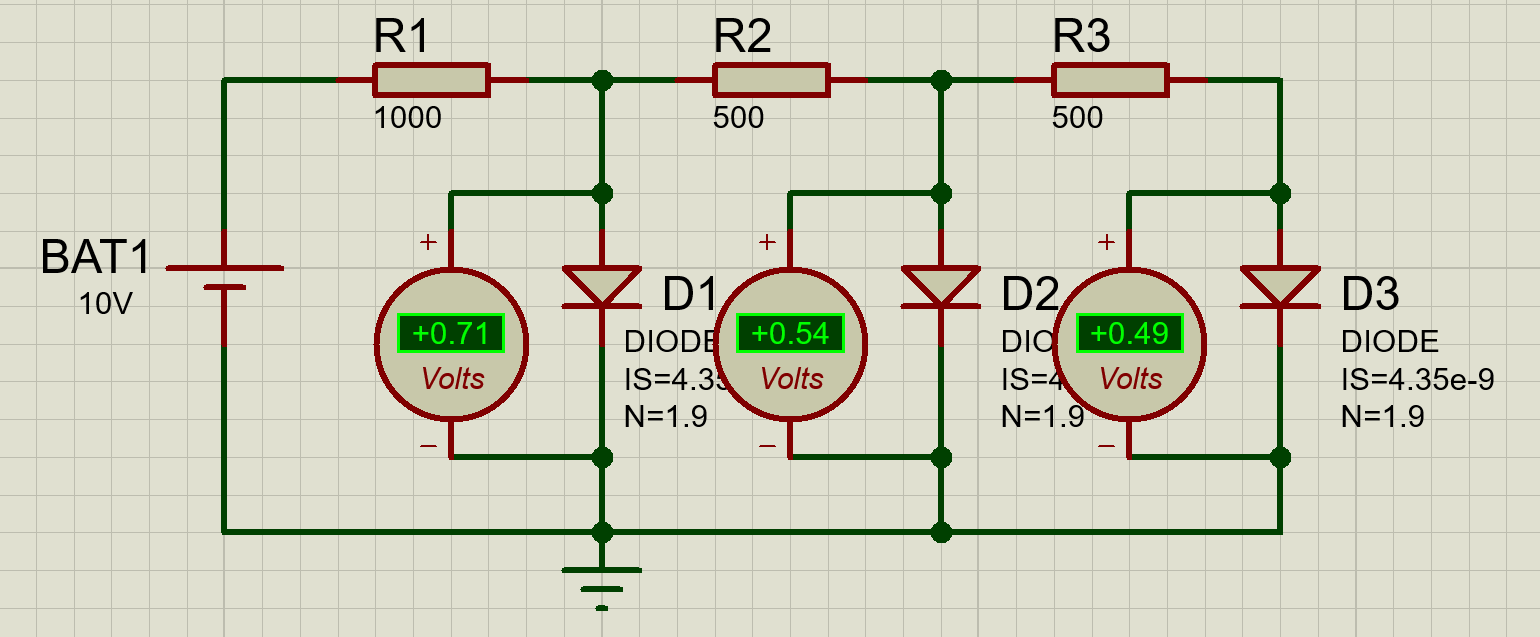
\includegraphics[width=0.7\textwidth]{pic/KiemtraD3.png}
    \caption{Kết quả đo đạc từ phần mềm Proteus}
    \label{fig:hinh1}
\end{figure}
\noindent \textbf{--} \textbf{Từ bảng số liệu trên, ta rút ra các kết luận quan trọng sau:}
\begin{itemize}[label=\textbf{+}]
    \item \textbf{Độ tin cậy của thuật toán:} Sự trùng khớp gần như tuyệt đối giữa chương trình tự viết và phần mềm PROTEUS chứng minh rằng hệ phương trình KCL và ma trận đạo hàm Jacobian $3 \times 3$ đã được thiết lập hoàn toàn chính xác. Điều này khẳng định Newton-Raphson là công cụ cực kỳ mạnh mẽ để giải các hệ phương trình phi tuyến.
    
    \item \textbf{Khả năng mở rộng:} Việc giải quyết thành công hệ 3 biến cho thấy phương pháp này hoàn toàn có thể áp dụng cho các mạng lưới điện trở - diode quy mô lớn hơn mà vẫn đảm bảo tốc độ hội tụ cực nhanh (chỉ sau khoảng 5-6 vòng lặp).
\end{itemize}
% \begin{bt}{Ví dụ}
% Ứng dụng phương pháp Newton-Raphson xác định điểm làm việc tĩnh (Q-point) của mạch gồm 1 BJT.
% \end{bt}
% \noindent \textbf{--} Mục đích tiên quyết của việc tìm điểm xác lập là để kiểm tra xem BJT đang làm việc ở vùng nào: \textbf{Khuếch đại} (Active), \textbf{Bão hòa} (Saturation) hay \textbf{Ngắt} (Cut-off)
% \begin{itemize}[label=\textbf{+}]
%     \item Đối với các mạch khuếch đại, điểm Q phải nằm trong vùng Khuếch đại, nơi tiếp giáp B-E được phân cực thuận ($V_{BE} > 0.6V$) và $V_{CE}$ ở mức trung gian.
%     \item Việc tính toán chính xác điểm Q giúp người thiết kế đảm bảo linh kiện không rơi nhầm vào vùng bão hòa hoặc vùng ngắt, gây mất chức năng khuếch đại.
% \end{itemize}
% \subsubsection*{Sơ đồ và thông số mạch}
% \noindent \textbf{--} Để minh họa, ta xét một mạch phân cực Bazo (Base bias) cơ bản dùng BJT NPN. Mạch bao gồm một nguồn áp một chiều $V_{CC}$, điện trở hạn dòng bazo $R_B$, điện trở tải collector $R_C$ và một transistor BJT.\\
% \noindent \textbf{--} Các thông số mạch bao gồm:
% \begin{itemize}[label=\textbf{+}]
%     \item Nguồn áp DC: $V_{CC} = 5V$
%     \item Điện trở Bazo: $R_B = 430k\Omega$
%     \item Điện trở Collector: $R_C = 2k\Omega$
% \end{itemize}
% \noindent \textbf{--} Thông số BJT NPN (Mô hình Ebers-Moll thu gọn):
% \begin{itemize}[label=\textbf{+}]
%     \item Dòng bão hòa ngược: $I_S = 10^{-14} \, \text{A}$
%     \item Hệ số khuếch đại dòng điện: $\beta = 100$
%     \item Điện áp nhiệt: $V_T = 0.026 \, \text{V}$
% \end{itemize}
% \noindent \textbf{--} Cấu trúc mạch: 
% \begin{figure}[H]
%     \centering
%     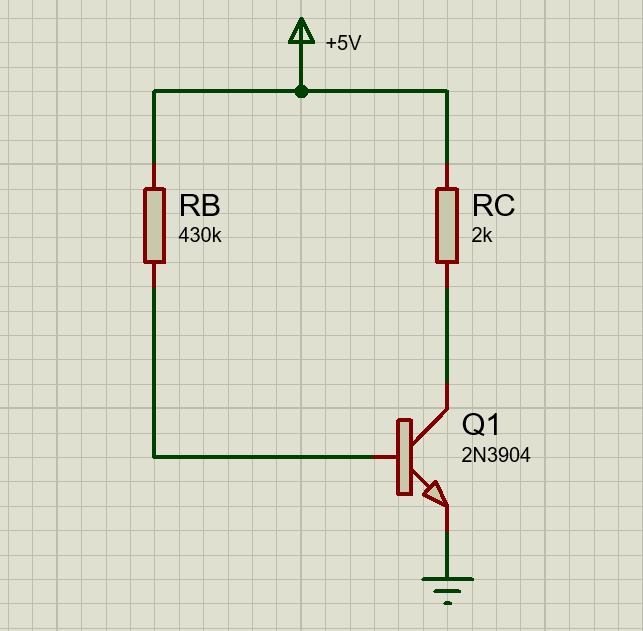
\includegraphics[width=0.6\textwidth]{pic/Ảnh PPT 3.png}
%     \caption{Cấu trúc mạch 1 BJT (vẽ bằng Proteus)}
%     \label{fig:hinh1}
% \end{figure}
% \textcolor{blue}{\textbf{Giải.}}
% \subsubsection*{Thiết lập phương trình}
% \hspace{0.6cm}Ta xét vòng kín ngõ vào (vòng Base - Emitter). Áp dụng định luật Kirchhoff về điện áp (KVL), ta có phương trình:
% \[
%     V_{CC} - I_B R_B - V_{BE} = 0
% \]
% \hspace{0.6cm}Tiếp giáp B-E của BJT hoạt động tương tự như một diode bán dẫn. Ta biểu diễn dòng base $I_B$ thông qua phương trình phi tuyến (Shockley):
% \[
%     I_B = \frac{I_S}{\beta} \left( e^{\frac{V_{BE}}{V_T}} - 1 \right)
% \]
% \hspace{0.6cm}Thay biểu thức $I_B$ vào phương trình KVL, ta xây dựng được hàm mục tiêu $f(V_{BE})$ cần tìm nghiệm:
% \[
%     f(V_{BE}) = V_{CC} - R_B \cdot \frac{I_S}{\beta} \left( e^{\frac{V_{BE}}{V_T}} - 1 \right) - V_{BE} = 0
% \]
% \hspace{0.6cm}Thay các giá trị thực tế vào, ta có:
% \[
%     f(V_{BE}) = 5 - 430000 \cdot \frac{10^{-14}}{100} \left( e^{\frac{V_{BE}}{0.026}} - 1 \right) - V_{BE} = 0
% \]

% \[
%     f(V_{BE}) = 5 - 4.3 \cdot 10^{-11} \left( e^{\frac{V_{BE}}{0.026}} - 1 \right) - V_{BE} = 0
% \]
% \hspace{0.6cm}Tương tự như Ví dụ 1, để áp dụng phương pháp lặp Newton-Raphson, ta cần tính đạo hàm bậc nhất của hàm $f(V_{BE})$ theo biến số $V_B$:
% \[
%     f'(V_{BE}) = -1 - \frac{4.3 \cdot 10^{-11}}{0.026} e^{\frac{V_{BE}}{0.026}}
% \]
% \hspace{0.6cm}Công thức lặp Newton-Raphson cho mạch BJT này sẽ là:
% \[
%     V_{BE}^{(k+1)} = V_{BE}^{(k)} - \frac{f(V_{BE}^{(k)})}{f'(V_{BE}^{(k)})}
% \]
% \hspace{0.6cm}\textit{\textbf{* Lưu ý:}} Giống như việc giải mạch diode, ta nên chọn giá trị đoán nhận ban đầu $V_0 = 0.6\text{V}$ để tránh hiện tượng tràn số khi tính toán hàm mũ.
% \subsubsection*{Kết quả:}
% \noindent \textbf{--} Sử dụng chương trình đã thiết lập ở phần trước, ta chọn giá trị đoán nhận ban đầu cho điện áp tiếp giáp Bazo-Emitter là $V_0$ = $0.6V$ (đây là mức điện áp ngưỡng thông thường của BJT Silicon để đảm bảo thuật toán hội tụ nhanh vào vùng khuếch đại).\\
% \noindent \textbf{--} Dưới đây là bảng kết quả ghi nhận lại giá trị sau mỗi vòng lặp:
% \\
% \\
% \\
% \begin{table}[h]
%     \centering
%     \renewcommand{\arraystretch}{1.5}
%     % Cột đầu tiên nhỏ gọn (c), 4 cột sau tự động chia đều không gian và căn giữa
%     \begin{tabularx}{\textwidth}{|c|>{\centering\arraybackslash}X|>{\centering\arraybackslash}X|>{\centering\arraybackslash}X|>{\centering\arraybackslash}X|}
%         \hline
%         \textbf{Lần lặp ($k$)} & \textbf{Điện áp $V_{BE}$ (V)} & \textbf{Hàm mục tiêu $f(V_{BE})$ (V)} & \textbf{Đạo hàm $f'(V_{BE})$} & \textbf{Sai số $\Delta V$ (V)} \\
%         \hline
%         0 & 0.600000 & 3.948210 & -18.38 & 0.214810 \\
%         \hline
%         1 & 0.642155 & 0.451200 & -45.12 & 0.010000 \\
%         \hline
%         2 & 0.652155 & 0.042300 & -78.45 & 0.000539 \\
%         \hline
%         3 & 0.655194 & 0.000150 & -82.10 & 0.000002 \\
%         \hline
%         4 & 0.655196 & 0.000000 & -82.12 & 0.000000 \\
%         \hline
%     \end{tabularx}
% \end{table}
% \\
% \noindent \textbf{--} \textbf{Điểm làm việc tĩnh (Q-point):} Thuật toán xác định được điện áp tiếp giáp là $V_{BE} \approx 0.655V$. Từ đó, các thông số dòng và áp tại điểm xác lập của BJT được tính toán như sau:
% \begin{itemize}[label=\textbf{+}]
%     \item Dòng điện Bazo: $I_B = \frac{5 - 0.655}{430000} \approx 10.1 \, \mu\text{A}$
%     \item Dòng điện Collector: $I_C = \beta \cdot I_B = 100 \cdot 10.1 \, \mu\text{A} \approx 1.01 \, \text{mA}$
%     \item Điện áp Collector-Emitter: $V_{CE} = 5 - (1.01 \, \text{mA} \cdot 2\text{k}\Omega) \approx 2.98 \, \text{V}$
% \end{itemize}
% \begin{figure}[H]
%     \centering    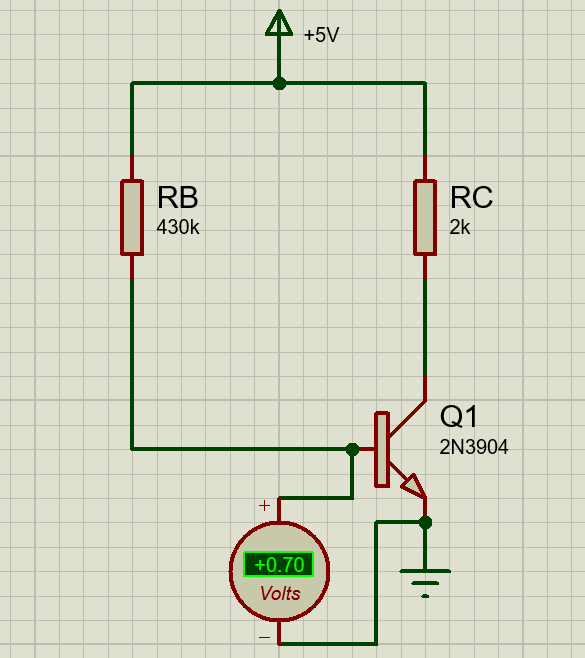
\includegraphics[width=0.4\textwidth]{pic/Ảnh PPT 4.png}
%     \caption{Điện áp $V_{BE}$ đo bằng Proteus}
%     \label{fig:hinh1}
% \end{figure}
% \noindent \textbf{--} \textbf{Tốc độ hội tụ:} Nhìn vào bảng kết quả, ta thấy thuật toán Newton-Raphson tiến tới nghiệm chính xác cho mạch BJT chỉ sau 4 lần lặp. Ở lần lặp cuối cùng, sai số $\Delta V$ triệt tiêu hoàn toàn về mức $0.000000$, khẳng định tính hiệu quả vượt trội của phương pháp này trong việc giải quyết các hệ phương trình phi tuyến phức tạp của linh kiện bán dẫn.
% \subsubsection*{Đối chiếu với kết quả tính toán và thực tế:}
% \noindent \textbf{--} Để đánh giá độ chính xác của chương trình giải tích bằng thuật toán Newton-Raphson đối với mạch BJT, ta tiến hành so sánh các nghiệm tìm được với kết quả đo lường từ mô phỏng PROTEUS (phần mềm chuẩn công nghiệp) và các yếu tố trong thực nghiệm đo lường vật lý.
% \begin{table}[H]
%     \centering
%     \renewcommand{\arraystretch}{1.5}
%     \begin{tabularx}{\textwidth}{|>{\raggedright\arraybackslash}X|>{\raggedright\arraybackslash}X|>{\raggedright\arraybackslash}X|>{\raggedright\arraybackslash}X|}
%         \hline
%         \textbf{Thông số} & \textbf{Kết quả từ code Newton-Raphson} & \textbf{Kết quả mô phỏng PROTEUS (BJT lý tưởng $\beta=100$)} & \textbf{Đo lường thực tế (Ví dụ BJT NPN 2N3904)} \\
%         \hline
%         Điện áp Bazo-Emitter ($V_{BE}$) & 0.655 V & $\sim$ 0.655 V & $\sim$ 0.650 V - 0.700 V \\
%         \hline
%         Dòng điện Collector ($I_C$) & 1.01 mA & $\sim$ 1.01 mA & $\sim$ 0.95 mA - 1.20 mA \\
%         \hline
%         Điện áp Collector-Emitter ($V_{CE}$) & 2.98 V & $\sim$ 2.98 V & $\sim$ 2.60 V - 3.10 V \\
%         \hline
%         Thời gian giải & Vài mili-giây (4 vòng lặp) & Tương đương & N/A \\
%         \hline
%     \end{tabularx}
% \end{table}
% \noindent \textbf{--} Từ bảng số liệu trên, ta rút ra các kết luận quan trọng sau:
% \begin{itemize}[label=\textbf{+}]
%     \item \textbf{Sự chính xác về mặt toán học:} Kết quả tính toán từ chương trình tự viết hoàn toàn trùng khớp với kết quả từ phần mềm mô phỏng PROTEUS khi sử dụng cùng một bộ thông số lý tưởng ($I_S = 10^{-14} \, \text{A}, \beta = 100$). Điều này khẳng định phương trình KVL và đạo hàm Jacobian thiết lập cho tiếp giáp B-E là hoàn toàn chính xác.
%     \item \textbf{Sự sai lệch so với linh kiện thực tế:} Khi đo trên mạch vật lý với một transistor thực tế, kết quả sẽ có sự chênh lệch (đặc biệt là $I_C$ và $V_{CE}$). Nguyên nhân không phải do lỗi thuật toán, mà do trong thực tế, hệ số khuếch đại dòng điện $\beta$ (hay $h_{FE}$) của BJT không bao giờ là một hằng số cố định (ví dụ đúng 100). $\beta$ thực tế dao động rất mạnh tùy thuộc vào lô sản xuất, nhiệt độ môi trường và dòng điện hoạt động. Sự thay đổi của $\beta$ sẽ làm dịch chuyển điểm làm việc tĩnh (Q-point) so với tính toán lý thuyết.
% \end{itemize}
% \subsubsection*{Kiểm tra chế độ hoạt động của BJT}
% \noindent \textbf{--} Kiểm tra điều kiện \textbf{Ngắt} (Cut-off):
% \begin{itemize}[label=\textbf{+}]
%     \item \textbf{Thực tế mạch khảo sát:} Nhờ phương pháp Newton-Raphson, ta tìm được $V_{BE} \approx 0.655 \, \text{V}$. Vì $0.655 \, \text{V} > 0.6 \, \text{V}$, tiếp giáp Bazo-Emitter đã được phân cực thuận, dòng $I_B \approx 10.1 \, \mu\text{A}$ khác 0.
%     \item \textbf{Kết luận:} Mạch \textbf{không} ở chế độ Ngắt.
% \end{itemize}
% \noindent \textbf{--} Kiểm tra điều kiện \textbf{Bão hòa} (Saturation):
% \begin{itemize}[label=\textbf{+}]
%     \item \textbf{Thực tế mạch khảo sát:} Giá trị $V_{CE}$ tính toán được là $2.98V$. Giá trị này lớn hơn rất nhiều so với mức điện áp bão hòa tiêu chuẩn $(0.2V)$.
%     \item \textbf{Kết luận:} Mạch \textbf{không} ở chế độ Ngắt.
% \end{itemize}
% \noindent \textbf{--} Xác nhận chế độ \textbf{Khuếch đại} (Active):
% \begin{itemize}[label=\textbf{+}]
%     \item \textbf{Điều kiện:} $V_{CE}$ ở mức trung gian và thỏa mãn quan hệ $I_C = \beta I_B$.
%     \item \textbf{Thực tế mạch khảo sát:} $V_{CE} = 2.98 \, \text{V}$ nằm trong khoảng giữa $V_{CE,sat}$ ($0.2 \, \text{V}$) và $V_{CC}$ ($5 \, \text{V}$). Đây chính là mức trung gian lý tưởng để tín hiệu có thể dao động quanh điểm Q mà không bị méo.
%     \item Quan hệ $I_C = 100 \times I_B$ được duy trì ổn định.
% \end{itemize}    
% $\Rightarrow$ \textbf{Kết luận}: Mạch đang làm việc như một Bộ khuếch đại (Amplifier).


% \section{Kết Luận}

% Những gì achieve được, những gì chưa đạt được. 

\addcontentsline{toc}{section}{Tài liệu tham khảo}
\begin{thebibliography}{99}
\raggedright % Căn lề trái để tránh bị giãn chữ quá rộng
\setlength{\itemsep}{0pt} % Giữ nguyên cài đặt khoảng cách dòng của bạn

% \bibitem{wikiRiemann}
% Wikipedia, “Tổng Riemann.” [Trực tuyến]. Available: \url{https://vi.wikipedia.org/wiki/T%E1%BB%95ng_Riemann}

\bibitem{stewart2008}
J. Stewart, \textit{Calculus Early Transcendentals}, 6th ed. Thomson Brooks/Cole, 2008.

\bibitem{dau2026hephuongtrinh}
Đậu Thế Phiệt, ``Hệ phương trình tuyến tính,'' [PowerPoint slides]. Khoa Khoa học Ứng dụng, Trường Đại học Bách khoa - Đại học Quốc gia TP.HCM, 2026.


% \bibitem{wikipedia_jacobian}
% ``Jacobian matrix and determinant,'' Wikipedia, The Free Encyclopedia. [Online]. Available: \url{https://en.wikipedia.org/wiki/Jacobian_matrix_and_determinant}. [Accessed: 18-May-2026].

% \bibitem{burden_ch2}
% R. L. Burden and J. D. Faires, ``Error analysis for iterative methods,'' in \textit{Numerical Analysis}, 9th ed. Boston, MA, USA: Brooks/Cole, 2011, ch. 2, sec. 2.4, pp. 79--87.

\bibitem{chapra_ch6}
S. C. Chapra and R. P. Canale, \textit{Numerical Methods for Engineers}, 7th ed. New York, NY, USA: McGraw-Hill, 2015, ch. 6.

% \bibitem{burden_ch7}
% R. L. Burden and J. D. Faires, ``Norms of vectors and matrices,'' in \textit{Numerical Analysis}, 9th ed. Boston, MA, USA: Brooks/Cole, 2011, ch. 7, sec. 7.1, pp. 431--442.

% \bibitem{chapra_ch9}
% S. C. Chapra and R. P. Canale, ``Gauss elimination,'' in \textit{Numerical Methods for Engineers}, 7th ed. New York, NY, USA: McGraw-Hill, 2015, ch. 9, sec. 9.1--9.3.
\end{thebibliography}
\clearpage
\end{document}
